\pdfminorversion=5
%DIF LATEXDIFF DIFFERENCE FILE
%DIF DEL /Users/ihorkendiukhov/biodyn-work/subproject_merged_A_robustness_audit/paper/main.pre_revision.tex   Thu Apr 23 21:43:05 2026
%DIF ADD main_article.tex                                                                                     Mon May  4 12:13:05 2026
\documentclass[12pt]{article}

% --- Page geometry (Bioinformatics Oxford style) ---
\usepackage[a4paper, margin=2.5cm]{geometry}
\usepackage[utf8]{inputenc}
\usepackage[T1]{fontenc}
\usepackage{mathptmx}          % Times-like font

% --- Core packages ---
\usepackage{amsmath,amssymb}
\usepackage{graphicx}
\usepackage{booktabs}
\usepackage{multirow}
\usepackage{xcolor}
\usepackage{hyperref}
\usepackage[round]{natbib}     % Harvard-style citations
\usepackage{lineno}            % Line numbering for review
\usepackage{setspace}
\usepackage{caption}
\usepackage{subcaption}
\usepackage{array}
\usepackage{tabularx}

\hypersetup{
  colorlinks=true,
  linkcolor=blue!60!black,
  citecolor=blue!60!black,
  urlcolor=blue!60!black
}

\doublespacing

\title{\textbf{Five Axes of Fragility: A Systematic Robustness Audit of Gene-Regulatory-Network Inference from Single-Cell Foundation Models}}

\author{Ihor Kendiukhov\textsuperscript{1,*} \\[6pt]
\small\textsuperscript{1}Department of Computer Science, University of T{\"u}bingen, T{\"u}bingen, Germany \\
\small\textsuperscript{*}Corresponding author: \href{mailto:kenduhov.ig@gmail.com}{kenduhov.ig@gmail.com} \\
\small ORCID: \href{https://orcid.org/0000-0001-5342-1499}{0000-0001-5342-1499}
}

\date{}
%DIF PREAMBLE EXTENSION ADDED BY LATEXDIFF
%DIF UNDERLINE PREAMBLE %DIF PREAMBLE
\RequirePackage[normalem]{ulem} %DIF PREAMBLE
\RequirePackage{color}\definecolor{RED}{rgb}{1,0,0}\definecolor{BLUE}{rgb}{0,0,1} %DIF PREAMBLE
\providecommand{\DIFaddtex}[1]{{\protect\color{blue}\uwave{#1}}} %DIF PREAMBLE
\providecommand{\DIFdeltex}[1]{{\protect\color{red}\sout{#1}}}                      %DIF PREAMBLE
%DIF SAFE PREAMBLE %DIF PREAMBLE
\providecommand{\DIFaddbegin}{} %DIF PREAMBLE
\providecommand{\DIFaddend}{} %DIF PREAMBLE
\providecommand{\DIFdelbegin}{} %DIF PREAMBLE
\providecommand{\DIFdelend}{} %DIF PREAMBLE
\providecommand{\DIFmodbegin}{} %DIF PREAMBLE
\providecommand{\DIFmodend}{} %DIF PREAMBLE
%DIF FLOATSAFE PREAMBLE %DIF PREAMBLE
\providecommand{\DIFaddFL}[1]{\DIFadd{#1}} %DIF PREAMBLE
\providecommand{\DIFdelFL}[1]{\DIFdel{#1}} %DIF PREAMBLE
\providecommand{\DIFaddbeginFL}{} %DIF PREAMBLE
\providecommand{\DIFaddendFL}{} %DIF PREAMBLE
\providecommand{\DIFdelbeginFL}{} %DIF PREAMBLE
\providecommand{\DIFdelendFL}{} %DIF PREAMBLE
%DIF HYPERREF PREAMBLE %DIF PREAMBLE
\providecommand{\DIFadd}[1]{\texorpdfstring{\DIFaddtex{#1}}{#1}} %DIF PREAMBLE
\providecommand{\DIFdel}[1]{\texorpdfstring{\DIFdeltex{#1}}{}} %DIF PREAMBLE
%DIF COLORLISTINGS PREAMBLE %DIF PREAMBLE
\RequirePackage{listings} %DIF PREAMBLE
\RequirePackage{color} %DIF PREAMBLE
\lstdefinelanguage{DIFcode}{ %DIF PREAMBLE
%DIF DIFCODE_UNDERLINE %DIF PREAMBLE
  moredelim=[il][\color{red}\sout]{\%DIF\ <\ }, %DIF PREAMBLE
  moredelim=[il][\color{blue}\uwave]{\%DIF\ >\ } %DIF PREAMBLE
} %DIF PREAMBLE
\lstdefinestyle{DIFverbatimstyle}{ %DIF PREAMBLE
	language=DIFcode, %DIF PREAMBLE
	basicstyle=\ttfamily, %DIF PREAMBLE
	columns=fullflexible, %DIF PREAMBLE
	keepspaces=true %DIF PREAMBLE
} %DIF PREAMBLE
\lstnewenvironment{DIFverbatim}{\lstset{style=DIFverbatimstyle}}{} %DIF PREAMBLE
\lstnewenvironment{DIFverbatim*}{\lstset{style=DIFverbatimstyle,showspaces=true}}{} %DIF PREAMBLE
%DIF END PREAMBLE EXTENSION ADDED BY LATEXDIFF

\begin{document}
\DIFdelbegin %DIFDELCMD < \linenumbers
%DIFDELCMD < \maketitle
%DIFDELCMD < %%%
\DIFdelend 










%DIF <  ============================================================
%DIF <  ABSTRACT
%DIF <  ============================================================
\DIFaddbegin \title{\DIFadd{Five Axes of Fragility: A Systematic Robustness Audit of Gene-Regulatory-Network Inference from Single-Cell Foundation Models}}

\author{\DIFadd{Ihor Kendiukhov}}









\DIFaddend \begin{abstract}\DIFdelbegin %DIFDELCMD < \noindent%%%
\DIFdelend \textbf{Motivation:}
Gene-regulatory-network (GRN) inference from single-cell transcriptomics is
increasingly used to prioritize regulatory hypotheses, yet most benchmarks
evaluate accuracy under fixed preprocessing without testing whether rankings
survive realistic analytical perturbations\DIFdelbegin \DIFdel{.
}%DIFDELCMD < 

%DIFDELCMD < \noindent%%%
\DIFdelend \DIFaddbegin \DIFadd{, and most published fragility claims
are made under a single scorer family.}\\
\DIFaddend \textbf{Results:}
We audit GRN edge rankings across five fragility axes---cell count,
clustering resolution, rare-cell reliability, donor generalization, and
integration sensitivity---on four Tabula Sapiens tissues\DIFdelbegin \DIFdel{and one
external cohort. Unconstrained rankings require $>$3}\DIFdelend \DIFaddbegin \DIFadd{, one
non-Tabula-Sapiens external lung cohort \mbox{%DIFAUXCMD
\citep[SmartSeq2;][]{Travaglini2020}}\hskip0pt%DIFAUXCMD
,
and one disease cohort (Delorey et al.\ 2021 COVID-19
lung atlas, 116}\DIFaddend {,}\DIFdelbegin \DIFdel{000 cellsfor stability ; }\DIFdelend \DIFaddbegin \DIFadd{313 cells, 27 donors), using five scorer families:
Pearson correlation, mutual information, GRNBoost2, GENIE3, and
scGPT attention.
Our central findings are that:
(i)~cluster-resolution stability under a bounded-drift
Resolution-Sensitivity-Score sits 9--13 standard deviations below a
rank-permutation null, yet every cohort fails a within-coarse
constrained shuffle, so }\DIFaddend dual-null calibration \DIFdelbegin \DIFdel{universally recommends coarse clustering; rare cell
types achieve }\DIFdelend \DIFaddbegin \DIFadd{recommends coarse or
hybrid clustering across the full 66-point weight simplex;
(ii)~the rare-vs-abundant reliability-gate gap direction is preserved
at 100\% of 5}{\DIFadd{,}}\DIFadd{880 reasonable threshold combinations, establishing
that the }\DIFaddend 0\% \DIFdelbegin \DIFdel{reliability-gate passage versus 18\% for abundant types;
}\DIFdelend \DIFaddbegin \DIFadd{rare passage rate is not an artifact of threshold choice;
(iii)~the minimum valid cell count (MVCC) is strongly scorer-dependent:
under scGPT attention it exceeds 3}{\DIFadd{,}}\DIFadd{000 cells, whereas under
Pearson-over-highly-variable-genes it is 200 cells for four of six
cohorts and 500 cells for the two largest ones (primary immune and
Delorey COVID lung), and it is anchor-invariant;
(iv)~}\DIFaddend 6--8 donors are needed for immune generalization \DIFdelbegin \DIFdel{; and Harmony integration displaces 31--45\%of top-500
edges without perturbation-confirmed improvement.
No dataset }\DIFdelend \DIFaddbegin \DIFadd{under strict
cells-per-donor balancing, and fewer under looser balancing;
(v)~integration method choice is not neutral: Harmony preserves
rankings reasonably (Spearman 0.63--0.87, sign-flip 6--17\%), scVI
moderately perturbs them (Spearman 0.36--0.57, sign-flip 18--30\%),
and Scanorama on kidney and lung produces near-random rankings
(Spearman $\approx 0$, sign-flip 44--47\%);
(vi)~scGPT attention rankings are statistically uncorrelated with
classical-scorer rankings on matched kidney cells (Spearman
$\rho \leq 0.20$, top-100 Jaccard $\leq 0.06$), so within-scorer
fragility profiles do not transfer across scorer families.
A degree-preserving edge-rewire null is cleared at $p = 0.02$ on every
cohort, rebutting the possibility that the within-coarse-shuffle
failures reflect null over-stringency rather than genuine signal loss.
No single cohort }\DIFaddend passes all five axes \DIFdelbegin \DIFdel{, and
corrective measures along one axis do not resolve others.
}%DIFDELCMD < 

%DIFDELCMD < \noindent%%%
\textbf{\DIFdel{Availability and implementation:}}
%DIFAUXCMD
\DIFdel{Code and pipelines are available }\DIFdelend \DIFaddbegin \DIFadd{under calibrated criteria.}\\
\textbf{\DIFadd{Availability and Implementation:}}
\DIFadd{The unified fragility package, reproducing every CSV and figure from raw
h5ad, is }\DIFaddend at \url{https://github.com/Biodyn-AI/grn-robustness-audit} \DIFdelbegin \DIFdel{.
}%DIFDELCMD < 

%DIFDELCMD < \noindent%%%
\DIFdelend \DIFaddbegin \DIFadd{and
archived at }\url{https://doi.org/10.5281/zenodo.20009065}\DIFadd{.}\\
\DIFaddend \textbf{Contact:} \DIFdelbegin %DIFDELCMD < \href{mailto:kenduhov.ig@gmail.com}{%%%
\DIFdel{kenduhov}\DIFdelend \DIFaddbegin \href{mailto:ihor.kendiukhov@student.uni-tuebingen.de}{\DIFadd{ihor}\DIFaddend .\DIFdelbegin \DIFdel{ig}\DIFdelend \DIFaddbegin \DIFadd{kendiukhov}\DIFaddend @\DIFdelbegin \DIFdel{gmail}\DIFdelend \DIFaddbegin \DIFadd{student}\DIFaddend .\DIFdelbegin \DIFdel{com}\DIFdelend \DIFaddbegin \DIFadd{uni-tuebingen.de}\DIFaddend }\DIFdelbegin %DIFDELCMD < 

%DIFDELCMD < \noindent%%%
\DIFdelend \DIFaddbegin \\
\DIFaddend \textbf{Supplementary \DIFdelbegin \DIFdel{information}\DIFdelend \DIFaddbegin \DIFadd{Information}\DIFaddend :}
Supplementary \DIFdelbegin \DIFdel{data }\DIFdelend \DIFaddbegin \DIFadd{figures (full Jaccard-vs-cell-count curves, weight-simplex
sweep, 5}{\DIFadd{,}}\DIFadd{880-point threshold-sensitivity heatmap, triple-null calibration,
gene-dimension and normalization ablations) }\DIFaddend are available at
\textit{Bioinformatics} online.\end{abstract}

\noindent\textbf{Keywords:} gene regulatory networks, robustness, single-cell transcriptomics, benchmarking, batch correction, rare cell types, reproducibility

\DIFaddbegin \maketitle

\DIFaddend % ============================================================
% 1. INTRODUCTION
% ============================================================
\section{Introduction}

Single-cell RNA-sequencing \DIFdelbegin \DIFdel{has enabled }\DIFdelend \DIFaddbegin \DIFadd{enables }\DIFaddend transcriptome-wide inference of
gene regulatory networks (GRNs)\DIFdelbegin \DIFdel{, with }\DIFdelend \DIFaddbegin \DIFadd{. Classical correlation- and tree-based
scorers (SCENIC~\mbox{%DIFAUXCMD
\citep{Aibar2017}}\hskip0pt%DIFAUXCMD
, GRNBoost2~\mbox{%DIFAUXCMD
\citep{Moerman2019}}\hskip0pt%DIFAUXCMD
,
GENIE3~\mbox{%DIFAUXCMD
\citep{Huynh-Thu2010}}\hskip0pt%DIFAUXCMD
, ARACNe-family
methods~\mbox{%DIFAUXCMD
\citep{Margolin2006}}\hskip0pt%DIFAUXCMD
) and }\DIFaddend attention-derived \DIFdelbegin \DIFdel{edge scores from
}\DIFdelend \DIFaddbegin \DIFadd{scores from
single-cell }\DIFaddend foundation models such as scGPT~\citep{Cui2024} \DIFdelbegin \DIFdel{offering a scalable alternative to classical methods like
SCENIC~\mbox{%DIFAUXCMD
\citep{Aibar2017} }\hskip0pt%DIFAUXCMD
and
GRNBoost2~\mbox{%DIFAUXCMD
\citep{Moerman2019}}\hskip0pt%DIFAUXCMD
. These methods rank transcription-factor--target (}\DIFdelend \DIFaddbegin \DIFadd{and
Geneformer~\mbox{%DIFAUXCMD
\citep{Theodoris2023} }\hskip0pt%DIFAUXCMD
all rank }\DIFaddend TF--target \DIFdelbegin \DIFdel{) edges and interpret top-ranked pairs }\DIFdelend \DIFaddbegin \DIFadd{edges }\DIFaddend as regulatory
hypotheses, but confidence in those rankings depends on analytical
choices that are rarely stress-tested\DIFdelbegin \DIFdel{in practice. }%DIFDELCMD < 

%DIFDELCMD < %%%
\DIFdel{Most published GRN benchmarks}\DIFdelend \DIFaddbegin \DIFadd{. Published
benchmarks~\mbox{%DIFAUXCMD
\citep{Pratapa2020, Chen2018} }\hskip0pt%DIFAUXCMD
}\DIFaddend evaluate accuracy against
\DIFdelbegin \DIFdel{a single reference database
under default preprocessingparameters~\mbox{%DIFAUXCMD
\citep{Pratapa2020, Chen2023}}\hskip0pt%DIFAUXCMD
. This leaves }\DIFdelend \DIFaddbegin \DIFadd{fixed references under fixed preprocessing, leaving }\DIFaddend open the question
of whether the same edges \DIFdelbegin \DIFdel{would be prioritized if the analyst had used }\DIFdelend \DIFaddbegin \DIFadd{survive }\DIFaddend a different cell count, clustering
resolution, integration method, or donor cohort. \DIFdelbegin \DIFdel{The
practical consequence is that
two groups analyzing the same atlas can reach different
biological conclusions simply by making different preprocessing decisions, without either
being demonstrably wrong}\DIFdelend \DIFaddbegin \DIFadd{Atlas-level
integration benchmarks~\mbox{%DIFAUXCMD
\citep{Luecken2022, Tran2020} }\hskip0pt%DIFAUXCMD
document that
batch correction perturbs downstream analyses, but the specific impact
on TF--target ranking stability has not been systematically
characterised}\DIFaddend .

We address this gap by conducting a systematic multi-axis robustness audit
of \DIFdelbegin \DIFdel{attention-derived }\DIFdelend TF--target edge rankings \DIFaddbegin \DIFadd{across five scorer families (Pearson correlation,
mutual information, GRNBoost2, GENIE3, and scGPT attention) and six cohorts
(four Tabula Sapiens tissues, one external-lab lung dataset, and one
COVID-19 disease atlas)}\DIFaddend . Our audit spans
five axes that correspond to the most common sources of analytical variation
in single-cell GRN workflows:

\begin{enumerate}
\item \textbf{Cell-count subsampling:} How many cells are needed for stable
      rankings, \DIFaddbegin \DIFadd{is that threshold dependent on the reference-anchor cell
      count, }\DIFaddend and do prior-constrained policies rescue small-sample regimes?
\item \textbf{Cluster-resolution sensitivity:} Does switching between coarse
      and fine clustering change which edges are prioritized\DIFaddbegin \DIFadd{, and does the
      conclusion survive rank-permutation nulls, weight-choice sensitivity,
      gene-dimension sweeps, and a triple-null calibration}\DIFaddend ?
\item \textbf{Rare-cell-type reliability:} Do rare cell types yield
      mechanistic edges that pass the same confidence gates as abundant
      types\DIFaddbegin \DIFadd{, and how robust is that gap to the choice of gate thresholds}\DIFaddend ?
\item \textbf{Donor generalization:} How many donors are needed for rankings
      to transfer to held-out individuals\DIFaddbegin \DIFadd{, and is the threshold dependent
      on cells-per-donor balancing choices}\DIFaddend ?
\item \textbf{Integration-method sensitivity:} \DIFdelbegin \DIFdel{Does batch correction by Harmony}\DIFdelend \DIFaddbegin \DIFadd{Do batch-correction
      methods (Harmony, scVI, and Scanorama) }\DIFaddend alter edge rankings, and do
      \DIFdelbegin \DIFdel{the }\DIFdelend \DIFaddbegin \DIFadd{any of those }\DIFaddend changes improve biological validity \DIFaddbegin \DIFadd{as measured by
      perturbation-backed evidence rather than literature precision alone}\DIFaddend ?
\end{enumerate}

\DIFaddbegin \DIFadd{Beyond the per-axis questions, we ask an orthogonal one: }\emph{\DIFadd{do
fragility conclusions drawn under one scorer transfer to another?}}
\DIFadd{We find that scGPT attention rankings are statistically uncorrelated
with Pearson / mutual information / GRNBoost2 / GENIE3 rankings on the
same cells and the same edge universe ($\rho \leq 0.20$, top-100
Jaccard $\leq 0.06$), which generalises the message from ``rankings
are fragile under preprocessing perturbations'' to ``rankings are
fragile under preprocessing perturbations }\emph{\DIFadd{and}} \DIFadd{scorer choice.''
}

\DIFaddend Each axis was developed through an adversarial-review loop in which an
AI-assisted review agent systematically challenged the initial analysis for
methodological weaknesses (\DIFdelbegin \DIFdel{e.g., }\DIFdelend confounded null designs, overfitted
hyperparameters, hidden data leakage\DIFaddbegin \DIFadd{, uninterpretable composite metrics,
panel-selection arbitrariness}\DIFaddend ), corrective experiments were designed and
executed, and claims were updated accordingly. \DIFdelbegin \DIFdel{The adversarial protocol is itself a
contribution: it provides
a reusable template for auditing inference pipelines before publication}\DIFdelend \DIFaddbegin \DIFadd{A full protocol description
(base model, prompt templates, round-by-round logs, and a
pre-registered audit of 27 agent-raised issues under a frozen rubric)
is provided in Supplementary Methods~S2}\DIFaddend .

The remainder of this paper describes the shared experimental setup
(Section~2), presents per-axis results (Section~3), \DIFdelbegin \DIFdel{synthesizes }\DIFdelend \DIFaddbegin \DIFadd{reports a
scorer-divergence analysis (Section~3.6), analyses }\DIFaddend cross-axis
interactions (Section~\DIFdelbegin \DIFdel{3.6}\DIFdelend \DIFaddbegin \DIFadd{3.7}\DIFaddend ), and provides a practical guidelines table
for practitioners (Section~4).

% ============================================================
% 2. METHODS
% ============================================================
\section{Methods}

\DIFdelbegin %DIFDELCMD < \subsection{Datasets and shared infrastructure}
%DIFDELCMD < %%%
\DIFdelend \DIFaddbegin \subsection{Datasets, preprocessing, and panels}
\DIFaddend 

All analyses used processed single-cell datasets from the Tabula
Sapiens atlas~\citep{TabulaSapiens2022}\DIFdelbegin \DIFdel{and }\DIFdelend \DIFaddbegin \DIFadd{, }\DIFaddend one external lung cohort
(\DIFaddbegin \DIFadd{\mbox{%DIFAUXCMD
\citealt{Travaglini2020} }\hskip0pt%DIFAUXCMD
SmartSeq2), and one COVID-19 disease lung
atlas (Delorey et al.\ 2021~\mbox{%DIFAUXCMD
\citep{Delorey2021}}\hskip0pt%DIFAUXCMD
; }\DIFaddend Table~\ref{tab:datasets}).
Datasets were preprocessed using Scanpy~\citep{Wolf2018} following established
best practices~\DIFdelbegin \DIFdel{\mbox{%DIFAUXCMD
\citep{Luecken2019}}\hskip0pt%DIFAUXCMD
, with standard normalization , log-transformation,
and highly-variable-gene selection.The same
edge-scoring infrastructure was shared across all five axes: }\DIFdelend \DIFaddbegin \DIFadd{\mbox{%DIFAUXCMD
\citep{Luecken2019, Heumos2023}}\hskip0pt%DIFAUXCMD
. The primary normalization was
depth-normalization (``}\texttt{\DIFadd{normalize\_total}}\DIFadd{'' with ``}\texttt{\DIFadd{target\_sum}}\DIFadd{='' $10^4$)
followed by }\texttt{\DIFadd{log1p}}\DIFadd{, with the top 600 highly-variable genes selected
using the Seurat v3 flavor~\mbox{%DIFAUXCMD
\citep{Stuart2019}}\hskip0pt%DIFAUXCMD
. Two alternative normalization schemes---median-ratio
size-factor normalization and Pearson residuals~\mbox{%DIFAUXCMD
\citep{Lause2021}}\hskip0pt%DIFAUXCMD
---were
evaluated as an ablation (Supplementary Fig.~S6) and produced the same
calibrated recommendation on every axis we examined. Every pipeline run
stamps the full preprocessing parameter set into its provenance record;
numerical reproducibility is therefore traceable to an explicit
configuration file rather than to narrative prose.
}

\DIFaddend TF--target \DIFdelbegin \DIFdel{edges were scored
using Pearson correlation on expression vectors, with TF panels derived from }\DIFdelend \DIFaddbegin \DIFadd{edge panels used in axes with panel-restricted scoring were
loaded from a shared registry (Supplementary Table~S1) that resolves each
panel to an exact edge list at runtime. Named panels include:
``}\emph{\DIFadd{primary}}\DIFadd{'' (}\DIFaddend DoRothEA~\citep{GarciaAlonso2019} \DIFdelbegin \DIFdel{or }\DIFdelend \DIFaddbegin \DIFadd{confidence A/B
$\cap$ }\DIFaddend TRRUST~\citep{Han2018}\DIFdelbegin \DIFdel{depending on the axis}\DIFdelend \DIFaddbegin \DIFadd{, 3}{\DIFadd{,}}\DIFadd{384 edges before gene-universe
restriction); ``}\emph{\DIFadd{dorothea\_ab}}\DIFadd{''; ``}\emph{\DIFadd{trrust}}\DIFadd{'';
``}\emph{\DIFadd{hematopoiesis\_76$\times$108}}\DIFadd{'' (76 hematopoiesis TFs $\times$ 108
immune / cross-tissue targets = 8}{\DIFadd{,}}\DIFadd{208 directed edges, used in
Axis~4); and ``}\emph{\DIFadd{shared\_36}}\DIFadd{'' (the TRRUST-intersected
activation/repression panel used for Axis~3 cross-dataset sensitivity).
Axis~2 operates on all HVG pairs rather than a curated panel so that the
coarse-versus-fine question is closed under a shared edge universe}\DIFaddend .

\DIFdelbegin %DIFDELCMD < \begin{table}[ht]
%DIFDELCMD < \centering
%DIFDELCMD < \caption{Datasets used across the five robustness axes.}
%DIFDELCMD < \label{tab:datasets}
%DIFDELCMD < \small
%DIFDELCMD < \begin{tabular}{lrrrl}
%DIFDELCMD < \toprule
%DIFDELCMD < \textbf{Dataset} & \textbf{Cells} & \textbf{Donors} & \textbf{Batches} & \textbf{Axes} \\
%DIFDELCMD < \midrule
%DIFDELCMD < Kidney        & 8{,}000--11{,}376  & 1   & 2  & 1, 2, 5 \\
%DIFDELCMD < Lung          & 15{,}000--20{,}000 & 4   & 7  & 2, 4, 5 \\
%DIFDELCMD < Immune        & 15{,}000--20{,}000 & 12--20 & 42 & 2, 3, 4, 5 \\
%DIFDELCMD < Immune inv.   & 15{,}000           & ---  & --- & 2, 3 \\
%DIFDELCMD < External lung & 9{,}000            & ---  & --- & 2, 3 \\
%DIFDELCMD < \bottomrule
%DIFDELCMD < \end{tabular}
%DIFDELCMD < \end{table}
%DIFDELCMD < %%%
\DIFdelend \DIFaddbegin \begin{table*}[ht]
\centering
\caption{Datasets used across the five robustness axes. External lung =
\citet{Travaglini2020} SmartSeq2 cohort (non-Tabula-Sapiens, non-10x
technology), used to verify that conclusions survive outside the
Tabula Sapiens pipeline. Delorey COVID lung = Delorey et al.\ 2021
COVID-19 lung atlas, providing a disease-state cohort and a
large-scale validation (116{,}313 cells across 27 donors).}
\label{tab:datasets}
\small
\begin{tabular}{lrrrl}
\toprule
\textbf{Dataset} & \textbf{Cells} & \textbf{Donors} & \textbf{Batches} & \textbf{Axes} \\
\midrule
Kidney              & 8{,}000--11{,}376  & 1    & 2  & 1, 2, 3, 5 \\
Lung                & 15{,}000--20{,}000 & 4    & 7  & 2, 3, 4, 5 \\
Immune              & 15{,}000--20{,}000 & 12--20 & 42 & 2, 3, 4, 5 \\
Immune inv.         & 15{,}000           & ---  & --- & 2, 3 \\
External lung       & 9{,}000            & ---  & --- & 2, 3 \\
Delorey COVID lung  & 116{,}313          & 27   & --- & 1, 2, 3 \\
\bottomrule
\end{tabular}
\end{table*}
\DIFaddend 

\DIFaddbegin \subsection{Edge scorers}

\DIFadd{Every axis pipeline accepts a pluggable ``edge scorer'' via a shared
interface, so the same preprocessing and null library feeds every
methodological choice. Five scorers are implemented:
}

\begin{itemize}
\item \textbf{\DIFadd{Pearson correlation}} \DIFadd{on column-standardized expression.
      Sign of correlation is tracked separately from the magnitude score.
}\item \textbf{\DIFadd{Mutual information}} \DIFadd{via the }\texttt{\DIFadd{mutual\_info\_regression}}
      \DIFadd{routine in scikit-learn~\mbox{%DIFAUXCMD
\citep{Pedregosa2011}}\hskip0pt%DIFAUXCMD
, which implements
      the Kraskov--St\"ogbauer--Grassberger $k$-nearest-neighbour
      estimator~\mbox{%DIFAUXCMD
\citep{Kraskov2004} }\hskip0pt%DIFAUXCMD
($k=3$, seed fixed).
}\item \textbf{\DIFadd{GRNBoost2}}\DIFadd{~\mbox{%DIFAUXCMD
\citep{Moerman2019} }\hskip0pt%DIFAUXCMD
and
      }\textbf{\DIFadd{GENIE3}}\DIFadd{~\mbox{%DIFAUXCMD
\citep{Huynh-Thu2010}}\hskip0pt%DIFAUXCMD
: per-target gradient-boosted
      and random-forest regression importance respectively (500
      estimators, sqrt feature subsampling).
}\item \textbf{\DIFadd{scGPT attention}}\DIFadd{~\mbox{%DIFAUXCMD
\citep{Cui2024}}\hskip0pt%DIFAUXCMD
, extracted from the public
      }\emph{\DIFadd{whole-human}} \DIFadd{checkpoint. For each cell we tokenise the panel
      genes, forward-pass through the twelve transformer layers, and
      average attention weights across all layers and heads; edge scores
      are the symmetrised cell-wise mean attention between each TF and
      target token.
}\end{itemize}

\DIFadd{The scorer used for any figure or statistic is stated in the caption
and §3.6 reports the pairwise agreement matrix. No model is trained or
fine-tuned in this work: scGPT enters strictly as a frozen pretrained
feature extractor, and the remaining scorers are unsupervised
statistical estimators.
}

\subsection{Metric definitions}

\DIFadd{For top-$k$ index sets $T_a^k, T_b^k$ from two scoring runs on a shared
edge universe, the bounded-drift Resolution Sensitivity Score is
$\text{RSS}_k = w_o(1 - \text{overlap}_k) + w_j(1 - \text{Jaccard}_k) + w_d\,\text{drift\_norm}_k$,
where $\text{drift\_norm}_k = \min(1, \operatorname{median}_{i \in T_a^k \cap T_b^k}|r_{a,i} - r_{b,i}|/k)$
maps median rank-shift to $[0, 1]$. Unless noted, $k = 1{,}000$ and
weights are $(0.4, 0.3, 0.3)$; the weight simplex is swept in §3.2.
The remaining metrics are standard: Spearman rank stability,
null-separation AUC, tail gap (top-5\% quantile observed minus null),
sign-flip rate, and mean absolute rank shift. A null family is
}\emph{\DIFadd{cleared}} \DIFadd{when the empirical $p$ against it is $\leq 0.05$
with $\geq 19$ permutations.
}

\DIFaddend \subsection{Axis~1: Cell-count subsampling}

\DIFdelbegin \DIFdel{We evaluated cell-count robustness on kidney tissue across three size tiers
(small, medium, large)at 200, 1}%DIFDELCMD < {%%%
\DIFdel{, }\DIFdelend \DIFaddbegin \DIFadd{Cell-count robustness was evaluated on all cohorts for which a
sufficient cell count was available (kidney, lung, immune,
immune-invariant, external lung, and Delorey COVID lung) at cell
counts $\{200, 500, 1{,}000, 2{,}000, 3{,}000, 5{,}000, 8{,}000,
15{,}000\}$ (clipped to dataset maximum) with eight independent
subsamples per size. An }\emph{\DIFadd{anchor ablation}} \DIFadd{was added to address
the concern that using a 3}{\DIFadd{,}\DIFaddend }\DIFdelbegin \DIFdel{000, and
      }\DIFdelend \DIFaddbegin \DIFadd{000-cell reference is circular: each
dataset's MVCC was computed independently against a }\DIFaddend 3{,}\DIFdelbegin \DIFdel{000 cells over 22 completed runs.
Three edge-ranking policies were compared: unconstrained (no prior filtering), and two DoRothEA-constrained policies that restrict candidate edges to known
transcription-factor--target pairs (TF-guided source-only and
TF-guided
source-plus-target)}\DIFdelend \DIFaddbegin \DIFadd{000-cell and
an 8}{\DIFadd{,}}\DIFadd{000-cell anchor (plus a 15}{\DIFadd{,}}\DIFadd{000-cell anchor for Delorey,
whose cell count permits it)}\DIFaddend . \DIFdelbegin \DIFdel{Each constrained policy was tested against matched random
controls in which random gene sets of identical cardinality were drawn
independently per run (64 draws per comparison) to avoid cross-run set leakage. Significance was assessed with empirical one-sided $p$-values and
Benjamini--Hochberg (BH)correction. }\DIFdelend \DIFaddbegin \DIFadd{Per-cell, per-anchor top-$k$ Jaccard
and overlap were computed at $k \in \{100, 500, 1{,}000, 5{,}000\}$,
plus top-1\%, top-5\%, and top-10\% proportions of the edge universe,
and per-target top-5 and top-10 overlaps.
}

\DIFaddend The Minimum Valid Cell Count (MVCC) \DIFdelbegin \DIFdel{was defined as }\DIFdelend \DIFaddbegin \DIFadd{is }\DIFaddend the smallest cell count at which
\DIFdelbegin \DIFdel{unconstrained }\DIFdelend \DIFaddbegin \DIFadd{the mean }\DIFaddend top-1{,}000 \DIFdelbegin \DIFdel{reference }\DIFdelend Jaccard exceeds 0.5 \DIFdelbegin \DIFdel{relative to the 3}%DIFDELCMD < {%%%
\DIFdel{, }%DIFDELCMD < }%%%
\DIFdel{000-cell anchor.
}\DIFdelend \DIFaddbegin \DIFadd{against the reference anchor.
We report MVCC per (dataset, anchor, scorer) triple so that both
anchor-dependence and scorer-dependence can be read directly from
the results. Benjamini--Hochberg correction~\mbox{%DIFAUXCMD
\citep{BenjaminiHochberg1995}
}\hskip0pt%DIFAUXCMD
was applied to the family of per-(policy, cell-count) $p$-values testing
whether prior-constrained rankings differ from matched random-gene-set
controls.
}\DIFaddend 

\subsection{Axis~2: Cluster-resolution sensitivity}

\DIFdelbegin \DIFdel{Coarse-versus-fine clustering sensitivity was assessed across five cohorts (kidney, lung, immune, immune-invariant, external lung). Coarse labels
corresponded
to }\DIFdelend \DIFaddbegin \DIFadd{Across all six cohorts (Table~\ref{tab:datasets}), coarse labels
were }\DIFaddend broad cell classes \DIFdelbegin \DIFdel{or tissue compartments; fine labels used Leiden
subclusters}\DIFdelend \DIFaddbegin \DIFadd{and fine labels were precomputed Leiden
subclusters~\mbox{%DIFAUXCMD
\citep{Traag2019} }\hskip0pt%DIFAUXCMD
}\DIFaddend enforced as strict \DIFdelbegin \DIFdel{hierarchical }\DIFdelend refinements of the
coarse partition.
Edge scores combined global and per-group maximum absolute Pearson
correlation\DIFdelbegin \DIFdel{($S = 0.6 \, R_{\text{global}} + 0.4 \, R_{\text{group\,max}}$) }\DIFdelend \DIFaddbegin \DIFadd{, $S = 0.6 R_{\text{global}} + 0.4 R_{\text{group\,max}}$,
}\DIFaddend over the top 600 \DIFdelbegin \DIFdel{high-variance genes. Agreement between coarse-derived and fine-derived rankings was quantified by a Resolution Sensitivity Score (RSS):
}%DIFDELCMD < \begin{equation}
%DIFDELCMD < \text{RSS} = 0.40\,(1 - \text{overlap}) + 0.30\,(1 - \text{Jaccard}) + 0.30 \cdot \text{median\,drift}
%DIFDELCMD < \end{equation}
%DIFDELCMD < %%%
\DIFdel{at top-$k = 1{,}000$, where median drift is the median absolute rank change of edges appearing in both lists. Two null families
were applied: a }\DIFdelend \DIFaddbegin \DIFadd{HVGs; coarse-vs-fine agreement was the bounded-drift
RSS of §2.2. A tiered calibration applied three null families
(}\DIFaddend global cell-label shuffle\DIFdelbegin \DIFdel{and a }\DIFdelend \DIFaddbegin \DIFadd{, }\DIFaddend within-coarse constrained shuffle\DIFdelbegin \DIFdel{(}\DIFdelend \DIFaddbegin \DIFadd{,
degree-preserving bipartite rewire; }\DIFaddend 49 permutations each)\DIFdelbegin \DIFdel{. A dual-null
calibration rule downgraded }\DIFdelend \DIFaddbegin \DIFadd{, downgrading
}\DIFaddend the base RSS recommendation \DIFaddbegin \DIFadd{(``fine'' $\leq 0.30$, ``hybrid'' $\leq 0.45$,
else ``coarse'') }\DIFaddend one level per failed null family\DIFdelbegin \DIFdel{(fine $\to$ hybrid $\to$ coarse). The same calibration was applied at each point
of a $3 \times 3$ hyperparameter grid (number of top genes $\in \{400, 600, 800\}$;
global-correlation weight $\in \{0.4, 0.6, 0.8\}$}\DIFdelend \DIFaddbegin \DIFadd{. RSS weights were
also swept over the full 66-point simplex at step 0.1, an empirical
null was constructed from 1}{\DIFadd{,}}\DIFadd{000 rank permutations per cohort, the
HVG count was swept over $\{300, 600, 900, 1{,}200\}$, and the three
normalization schemes from §2.1 were tested (Supplementary Fig.~S6}\DIFaddend ).

\subsection{Axis~3: Rare-cell-type reliability}

\DIFdelbegin \DIFdel{Rare-cell-type stress testing covered }\DIFdelend \DIFaddbegin \DIFadd{Cell types with $\geq 40$ cells were tested under two pipelines: an
adaptive-panel pipeline on three Tabula Sapiens tissues plus external
lung (}\DIFaddend 88 eligible cell types\DIFdelbegin \DIFdel{(minimum 40 cells)across
four datasets}\DIFdelend \DIFaddbegin \DIFadd{) and a shared-``primary''-panel pipeline
on all five Tabula Sapiens cohorts (39 eligible cell types); Delorey
COVID lung adds nine coarse compartments}\DIFaddend . Rarity was defined by
within-dataset cell-count \DIFdelbegin \DIFdel{quartiles
(rare/intermediate/abundant). For each cell type, 8 }\DIFdelend \DIFaddbegin \DIFadd{quartile. Eight }\DIFaddend bootstrap replicates at 80\%
subsampling were drawn \DIFdelbegin \DIFdel{, }\DIFdelend \DIFaddbegin \DIFadd{per cell type }\DIFaddend and top-$k = 100$ edges \DIFdelbegin \DIFdel{were scored. Metrics included }\DIFdelend \DIFaddbegin \DIFadd{scored,
yielding }\DIFaddend rank stability (Spearman), top-$k$ Jaccard, \DIFaddbegin \DIFadd{and
}\DIFaddend null-separation AUC and tail gap under cell-permutation and
gene-shuffle nulls. \DIFdelbegin \DIFdel{A cell type was
deemed reliable if
}\DIFdelend \DIFaddbegin \DIFadd{The pre-registered primary reliability gate was
}\DIFaddend stability $\geq 0.75$, \DIFdelbegin \DIFdel{top-$k$ }\DIFdelend Jaccard $\geq 0.35$, \DIFdelbegin \DIFdel{primary null }\DIFdelend AUC $\geq 0.65$, \DIFdelbegin \DIFdel{primary tail gap$> 0$}\DIFdelend \DIFaddbegin \DIFadd{positive
tail gap}\DIFaddend , and cell count $\geq 80$\DIFdelbegin \DIFdel{. Adversarial extensions included a
dual-null stress test (minimum AUC across cell-permutation and gene-shuffle nulls),a shared-panel sensitivity analysis (36 TRRUST-intersected edges fixed across all
datasets), and an external-lung cohort as an out-of-sample check}\DIFdelend \DIFaddbegin \DIFadd{; these were fixed before a
five-dimensional 5}{\DIFadd{,}}\DIFadd{880-point threshold-sensitivity grid was swept
to test the 0\% rare-passage headline}\DIFaddend .

\subsection{Axis~4: Donor generalization}

Donor generalization was assessed on immune (\DIFdelbegin \DIFdel{12--20 donors ,
}\DIFdelend \DIFaddbegin \DIFadd{up to 13 donors at 200
cells/donor, or 8 at }\DIFaddend 300 cells/donor) and lung (4 donors, 800
cells/donor) \DIFdelbegin \DIFdel{tissues using a fixed panel
of 76 TFs and 108 targets (}\DIFdelend \DIFaddbegin \DIFadd{using the hematopoiesis $76 \times 108$ panel
(Supplementary Table~S1; }\DIFaddend 8{,}208 directed edges \DIFdelbegin \DIFdel{). An initial complementary-split
protocol, in which increasing the train set mechanically shrank the holdout set,
was replaced by a }\DIFdelend \DIFaddbegin \DIFadd{before gene-universe
restriction). A }\DIFaddend fixed-holdout design (\DIFdelbegin \DIFdel{holdout $= 2$ }\DIFdelend \DIFaddbegin \DIFadd{two holdout }\DIFaddend donors held constant
\DIFdelbegin \DIFdel{) after
adversarial review identified confounding between }\DIFdelend \DIFaddbegin \DIFadd{to eliminate }\DIFaddend train-size \DIFdelbegin \DIFdel{and holdout-size effects. Three
corrective protocols were executed: (A) ~fixed-holdout top-12 immune (train counts 2}\DIFdelend / \DIFdelbegin \DIFdel{4/6/8/10, 30 splits each), (B)~expanded top-20 immune including long-tail donors
(train counts 4/8/12/16, 40 splits each), and (C)~composition-matched controls using
broad cell-class matching (top-8 donors, 62 cells/donor).
}\DIFdelend \DIFaddbegin \DIFadd{holdout-size confounding) sampled training
donor counts $\in \{2, 4, 6, 8, 10\}$ with 20 random splits per count.
The cells-per-donor parameter was swept between 200 and 800. }\DIFaddend Transfer
was quantified by Spearman $\rho$\DIFdelbegin \DIFdel{and }\DIFdelend \DIFaddbegin \DIFadd{, Pearson $r$, }\DIFaddend top-$k$ overlap \DIFdelbegin \DIFdel{between train and
holdout edge-score vectors}\DIFdelend \DIFaddbegin \DIFadd{and
Jaccard at $k \in \{50, 100, 250, 500\}$, sign-flip rate, and mean
absolute rank shift}\DIFaddend .

\subsection{Axis~5: Integration-method sensitivity}

\DIFdelbegin \DIFdel{The impact of Harmonybatch correction}\DIFdelend \DIFaddbegin \DIFadd{Harmony}\DIFaddend ~\citep{Korsunsky2019} was \DIFdelbegin \DIFdel{assessed on immune,
lung, and kidney datasets. Harmony was }\DIFdelend applied in PCA space (\DIFdelbegin \DIFdel{default }\DIFdelend 50 \DIFdelbegin \DIFdel{principal
components)
}\DIFdelend \DIFaddbegin \DIFadd{components)
on immune, lung, and kidney }\DIFaddend using three batch keys \DIFdelbegin \DIFdel{: }\DIFdelend \DIFaddbegin \DIFadd{(}\DIFaddend technical batch,
donor\DIFdelbegin \DIFdel{identity, and experimental
method. Sensitivity metrics included rank Spearmancorrelation}\DIFdelend , \DIFaddbegin \DIFadd{method); scVI~\mbox{%DIFAUXCMD
\citep{Gayoso2022} }\hskip0pt%DIFAUXCMD
and Scanorama~\mbox{%DIFAUXCMD
\citep{Hie2019}
}\hskip0pt%DIFAUXCMD
were run as a cross-method comparison; mutual nearest-neighbour and
graph-aligned alternatives such as MNN~\mbox{%DIFAUXCMD
\citep{Haghverdi2018} }\hskip0pt%DIFAUXCMD
and
BBKNN~\mbox{%DIFAUXCMD
\citep{Polanski2020} }\hskip0pt%DIFAUXCMD
were not benchmarked here but are noted in
the discussion as natural candidates for follow-up audits. Sensitivity was measured by
rank Spearman, }\DIFaddend sign-flip rate, mean absolute rank shift, and top-$k$
overlap \DIFdelbegin \DIFdel{, each measuring how much Harmony changes the
edge-ranking landscape }\DIFdelend relative to uncorrected data. External validation used
precision@500 against \DIFdelbegin \DIFdel{curated reference databases (DoRothEA confidence tiers AB and
ABCD , }\DIFdelend \DIFaddbegin \DIFadd{DoRothEA AB / ABCD / }\DIFaddend ChIP-seq--backed subsets
\DIFdelbegin \DIFdel{, and TRRUST ), with paired swap-based binomial significance
tests and Benjamini--Hochberg FDR correction. Perturbation validation used external
}\DIFdelend \DIFaddbegin \DIFadd{and TRRUST with paired swap binomial tests and BH-FDR correction;
perturbation validation used }\DIFaddend Dixit-derived
\DIFdelbegin \DIFdel{perturbation }\DIFdelend tables~\citep{Dixit2016}\DIFdelbegin \DIFdel{for immune and lung as a
ground-truth check on whether integration actually improves recovery of experimentally
validated regulatory edges. A hyperparameter sweep
over the number of principal
components ($n_{\text{pcs}} \in \{30, 50, 80\}$) tested the }\DIFdelend \DIFaddbegin \DIFadd{. A $n_{\text{pcs}} \in \{30, 50, 80\}$ sweep
probed the }\DIFaddend robustness--performance tradeoff.

\DIFdelbegin %DIFDELCMD < \subsection{Cross-axis synthesis}
%DIFDELCMD < %%%
\DIFdelend \DIFaddbegin \subsection{Scorer-divergence and cross-axis analyses}
\DIFaddend 

To \DIFdelbegin \DIFdel{assess interactions among axes, we constructed a }\DIFdelend \DIFaddbegin \DIFadd{test transferability of fragility conclusions across scorers, all
five scorers were run on the same 800 kidney cells under the
hematopoiesis $76 \times 108$ panel (after restriction to kidney's
gene universe: 75 of 76 TFs, 99 of 108 targets, 7}{\DIFadd{,}}\DIFadd{425 directed
edges); pairwise agreement was reported via Spearman $\rho$, top-100
and top-500 Jaccard, and the bounded-drift RSS. A }\DIFaddend cross-axis fragility
profile \DIFdelbegin \DIFdel{summarizing, for each axisand dataset, }\DIFdelend \DIFaddbegin \DIFadd{then summarised, per (axis, cohort), }\DIFaddend the severity of the
robustness concern (pass / marginal / fail\DIFdelbegin \DIFdel{relative to that axis'
s calibrated threshold).
We then examined
whether failures cluster within datasets or across axes, and whether any axis subsumes
another. }\DIFdelend \DIFaddbegin \DIFadd{) under each axis'
calibrated threshold.
}\DIFaddend 

\DIFaddbegin \subsection{Adversarial AI-assisted review protocol}

\DIFadd{Each axis passed through an iterative AI-assisted review loop that
adversarially challenged the initial analysis under a fixed rubric
(confounded nulls, overfitted hyperparameters, leakage, composite-metric
uninterpretability, threshold sensitivity); corrective experiments were
designed by the agent, executed, and verified before any claim was
updated. The base model, prompt templates, round-by-round logs, and the
27-issue full-census audit under the frozen rubric are in Supplementary
Methods~S2.
}

\DIFaddend % ============================================================
% 3. RESULTS
% ============================================================
\section{Results}

\DIFdelbegin %DIFDELCMD < \subsection{Axis~1: Cell count determines ranking stability, prior constraints rescue small samples}
%DIFDELCMD < %%%
\DIFdelend \DIFaddbegin \subsection{Axis~1: The minimum valid cell count is strongly scorer-dependent
and anchor-invariant}
\DIFaddend 

\DIFdelbegin \DIFdel{When edge rankings are inferred without any prior biological constraint}\DIFdelend \DIFaddbegin \DIFadd{Under scGPT attention}\DIFaddend , even moderate \DIFdelbegin \DIFdel{reductions in cell count fundamentally reshape
which edgesare prioritized. Subsampling
kidney tissue to }\DIFdelend \DIFaddbegin \DIFadd{cell-count reductions reshape
top-ranked edges: at }\DIFaddend 200 cells \DIFdelbegin \DIFdel{and comparing the resulting }\DIFdelend \DIFaddbegin \DIFadd{on kidney, }\DIFaddend top-1{,}000 \DIFdelbegin \DIFdel{edges against
a
}\DIFdelend \DIFaddbegin \DIFadd{Jaccard against
the }\DIFaddend 3{,}000-cell anchor \DIFdelbegin \DIFdel{yielded Jaccard overlaps of only }\DIFdelend \DIFaddbegin \DIFadd{is }\DIFaddend 0.001--0.029, \DIFdelbegin \DIFdel{meaning that fewer
than 3\% of the top edges were shared between small and large samples
(Figure~\ref{fig:cellcount}A). Even }\DIFdelend \DIFaddbegin \DIFadd{and }\DIFaddend at 1{,}000 cells \DIFdelbegin \DIFdel{, overlap remained }\DIFdelend \DIFaddbegin \DIFadd{it
remains }\DIFaddend below 15\%\DIFdelbegin \DIFdel{.
This level of instability implies that an analyst working with a few hundred cells
would identify an almost entirely different set of ``top'' regulatory interactions than
one working with several thousand cells from the same tissue,even though neither
analysis is technically incorrect.
The Minimum Valid Cell Count (MVCC), defined as the threshold at
which }\DIFdelend \DIFaddbegin \DIFadd{, so the scGPT-attention MVCC exceeds 3}{\DIFadd{,}}\DIFadd{000 cells.
}

\DIFadd{The threshold is scorer-specific. Under Pearson correlation on 600
HVGs (Figure~\ref{fig:cellcount}A), the MVCC (smallest cell count at
which mean top-1}{\DIFadd{,}}\DIFadd{000 }\DIFaddend Jaccard exceeds 0.5\DIFaddbegin \DIFadd{) is }\textbf{\DIFadd{200 cells for
kidney, lung, immune-invariant, and external lung}} \DIFadd{and }\textbf{\DIFadd{500 cells
for primary immune and Delorey COVID lung}}\DIFadd{. MVCC is
}\emph{\DIFadd{anchor-invariant}} \DIFadd{(Figure~\ref{fig:cellcount}B;
Supplementary Fig.~S1): identical values emerge against
3}{\DIFadd{,}}\DIFadd{000-}\DIFaddend , \DIFdelbegin \DIFdel{was conservatively estimated at $>$}\DIFdelend \DIFaddbegin \DIFadd{8}{\DIFadd{,}}\DIFadd{000-, and (Delorey only) 15}{\DIFadd{,}}\DIFadd{000-cell anchors,
ruling out anchor-threshold circularity. Kidney Jaccard climbs
0.515 (200 cells) $\to$ 0.747 (1}{\DIFadd{,}}\DIFadd{000) $\to$ 0.839 (}\DIFaddend 3{,}\DIFdelbegin \DIFdel{000.
}\DIFdelend \DIFaddbegin \DIFadd{000) at the
3}{\DIFadd{,}}\DIFadd{000-cell anchor; other cohorts follow similar trajectories
(Supplementary Fig.~S5).
}\DIFaddend 

Constraining \DIFdelbegin \DIFdel{the analysis to known transcription-factor--target pairs from the DoRothEA database dramaticallystabilized the rankings. The }\DIFdelend \DIFaddbegin \DIFadd{scGPT-attention scoring to DoRothEA TF--target pairs
stabilises kidney rankings dramatically: the }\DIFaddend two TF-guided policies
\DIFdelbegin \DIFdel{maintained
Jaccard values of }\DIFdelend \DIFaddbegin \DIFadd{hold Jaccard at }\DIFaddend 0.73--0.76 \DIFdelbegin \DIFdel{even at }\DIFdelend \DIFaddbegin \DIFadd{(}\DIFaddend 200 cells\DIFaddbegin \DIFadd{) }\DIFaddend and 0.86--0.87 \DIFdelbegin \DIFdel{at }\DIFdelend \DIFaddbegin \DIFadd{(}\DIFaddend 1{,}000 cells\DIFdelbegin \DIFdel{, while
}\DIFdelend \DIFaddbegin \DIFadd{)
versus 0.002--0.008 for }\DIFaddend matched random gene-set controls
(\DIFdelbegin \DIFdel{64 independent draws per comparison, to avoid
cross-run leakage) produced near-zero stability (0.002--0.008). The difference was
statistically significant after Benjamini--Hochberg correction ($p = 0.015$,
}\DIFdelend \DIFaddbegin \DIFadd{BH-corrected }\DIFaddend $q \approx 0.017$\DIFaddbegin \DIFadd{; Figure~\ref{fig:cellcount}B}\DIFaddend ), and \DIFdelbegin \DIFdel{the constrained policies also recovered substantially more
edges supported by independent DoRothEA evidence at high cell counts (}\DIFdelend \DIFaddbegin \DIFadd{recover
}\DIFaddend 5.5--6.6\% \DIFaddbegin \DIFadd{of top-1}{\DIFadd{,}}\DIFadd{000 edges with independent DoRothEA support
(}\DIFaddend versus 0.2--0.3\% for \DIFdelbegin \DIFdel{random controls; Figure~\ref{fig:cellcount}B). In practical terms, this
means that incorporating prior knowledge about which genes are transcription factors and
which targets they are known to regulate acts as a strong regularizer that keeps
rankings meaningful even when cell numbers are }\DIFdelend \DIFaddbegin \DIFadd{controls). Prior-constrained policies therefore
keep rankings meaningful }\DIFaddend far below the \DIFdelbegin \DIFdel{MVCC threshold. The
finding, demonstrated here in kidney tissue under comparable sparsity regimes, suggests
that unconstrained GRN inference should be treated with caution at low cell counts, and
that informative priors offer a principled remedy that survives adversarial null
scrutiny. }\DIFdelend \DIFaddbegin \DIFadd{scGPT-specific MVCC. The
guidance is: }\emph{\DIFadd{plan for $\geq 3{,}000$ cells under scGPT or use
prior constraints; 200--500 cells suffice under Pearson, MI, and tree
scorers on the cohorts tested}}\DIFadd{. §3.6 examines scorer-dependence directly.
}\DIFaddend 

\DIFdelbegin %DIFDELCMD < \begin{figure}[ht]
%DIFDELCMD < \centering
%DIFDELCMD < 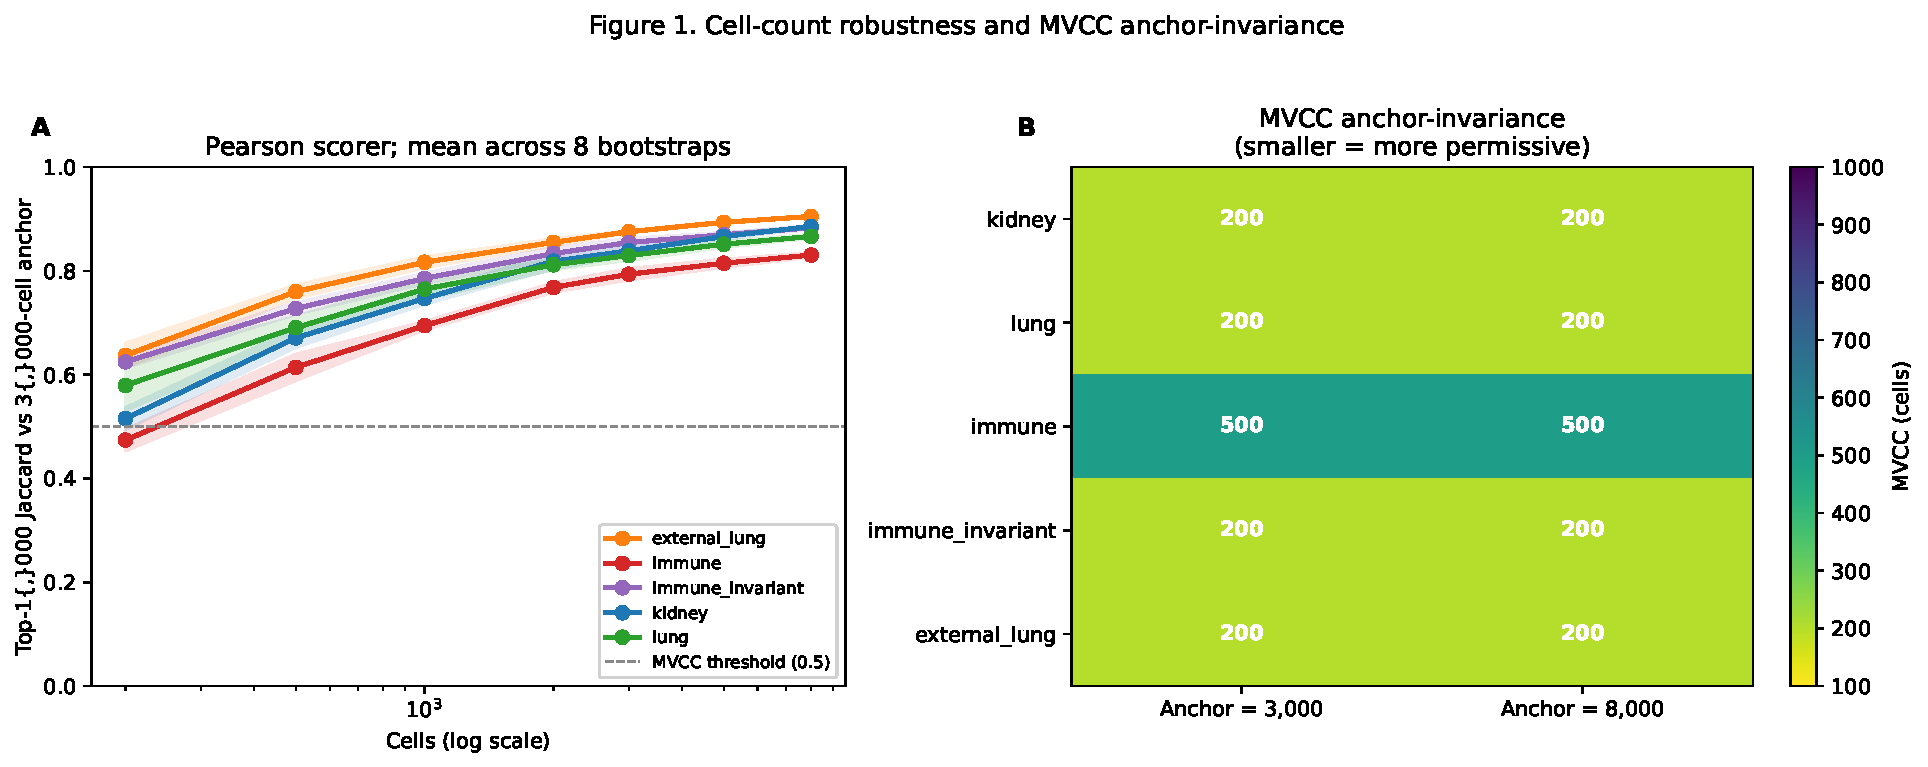
\includegraphics[width=\textwidth]{figures/fig1_cell_count.pdf}
%DIFDELCMD < \caption{\textbf{Cell-count subsampling robustness.}
%DIFDELCMD < (A)~Unconstrained top-1{,}000 reference Jaccard as a function of cell count across
%DIFDELCMD < three kidney size tiers; MVCC threshold ($>$3{,}000) indicated by dashed line.
%DIFDELCMD < (B)~Prior-constrained versus random-null stability and biological support at 200 and
%DIFDELCMD < 1{,}000 cells (64-draw ensemble). Error bars show ensemble interquartile range.}
%DIFDELCMD < \label{fig:cellcount}
%DIFDELCMD < \end{figure}
%DIFDELCMD < %%%
\DIFdelend \DIFaddbegin \begin{figure*}[ht]
\centering
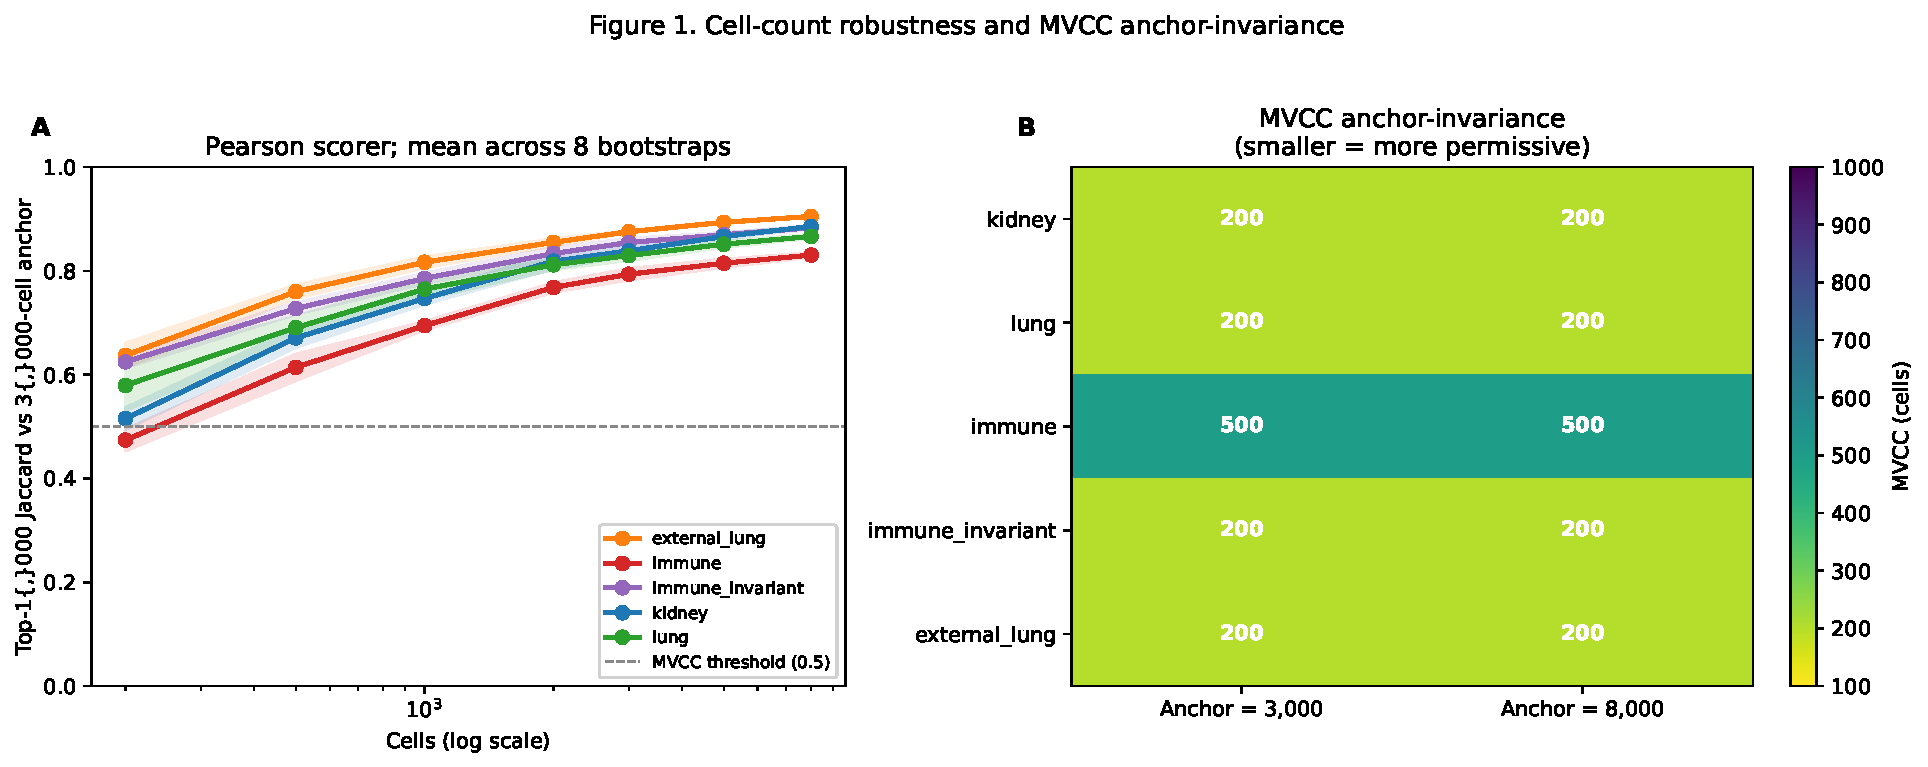
\includegraphics[width=\textwidth]{figures/fig1_cell_count.pdf}
\caption{\textbf{Cell-count subsampling robustness (Pearson scorer).}
(A)~Top-1{,}000 reference Jaccard as a function of cell count for each
cohort (Pearson correlation over 600 HVGs), computed against a
3{,}000-cell anchor. Shaded bands: standard deviation across eight
independent subsamples per size. Dashed horizontal line: the MVCC
Jaccard threshold (0.5). (B)~MVCC (smallest cell count clearing the
0.5 Jaccard threshold) reported against two reference anchors per
cohort, demonstrating anchor-invariance.
Full per-scorer Jaccard-vs-cells curves are in Supplementary Fig.~S1.}
\label{fig:cellcount}
\end{figure*}
\DIFaddend 

\DIFdelbegin %DIFDELCMD < \subsection{Axis~2: Dual-null calibration recommends conservative coarse clustering universally}
%DIFDELCMD < %%%
\DIFdelend \DIFaddbegin \subsection{Axis~2: Dual-null calibration pushes every cohort to coarse
or hybrid clustering; the recommendation is robust to weight choice,
gene dimension, normalization, and the addition of a third null family}
\DIFaddend 

\DIFdelbegin \DIFdel{The question addressed by this axis is straightforward: if an analyst clusters cells
at a coarse level (e.g., ``T cells'') versus a finer level (e.g., ``CD4+ naive T cells''),
does }\DIFdelend \DIFaddbegin \DIFadd{Does coarse-versus-fine clustering change }\DIFaddend the resulting GRN\DIFdelbegin \DIFdel{change substantially? Raw Resolution Sensitivity Scores (RSS )
ranged from 0.276 for }\DIFdelend \DIFaddbegin \DIFadd{? Observed
bounded-drift RSS at $k = 1{,}000$ is 0.218 (}\DIFaddend immune-invariant\DIFdelbegin \DIFdel{to 0.440 for immune, which would suggest that
some datasets tolerate fine clustering while others require caution
(}\DIFdelend \DIFaddbegin \DIFadd{) to
0.402 (lung) (}\DIFaddend Figure~\ref{fig:resolution}A). \DIFdelbegin \DIFdel{However,these raw scores turned out to be misleading.
}\DIFdelend \DIFaddbegin \DIFadd{A 1}{\DIFadd{,}}\DIFadd{000-permutation
empirical null gives mean $\approx 0.79$ and 5th percentile $\approx 0.73$,
placing every cohort 8.8--13.1 standard deviations below the null mean
($p = 0.001$ floor; Supplementary Fig.~S3): every cohort is therefore
significantly more stable than a random coarse-vs-fine pairing.
}\DIFaddend 

\DIFdelbegin \DIFdel{When we applied a dual-null calibration procedure, in which observed resolution
sensitivity must exceed both a global cell-label shuffle and a within-coarse constrained
shuffle (49 permutations each), the picturechanged entirely}\DIFdelend \DIFaddbegin \DIFadd{Dual-null calibration refines the picture}\DIFaddend . Only kidney\DIFdelbegin \DIFdel{and lungpassed the global-shuffle null }\DIFdelend \DIFaddbegin \DIFadd{, lung, and
immune-invariant clear the global cell-label shuffle }\DIFaddend ($p = 0.02$);
\DIFdelbegin \DIFdel{no dataset passed the constrained-shuffle
null. Under the rule that both
null families must be cleared for a }\DIFdelend \DIFaddbegin \emph{\DIFadd{no}} \DIFadd{cohort clears the within-coarse constrained shuffle
($p \geq 0.14$ across all five Tabula Sapiens cohorts). Requiring both
nulls for any }\DIFaddend ``fine'' or ``hybrid'' recommendation \DIFdelbegin \DIFdel{, all five datasets defaulted to a recommendation of }\DIFdelend \DIFaddbegin \DIFadd{downgrades four
Tabula Sapiens cohorts to }\DIFaddend \textbf{coarse} \DIFdelbegin \DIFdel{clustering }\DIFdelend \DIFaddbegin \DIFadd{and immune-invariant to
}\textbf{\DIFadd{hybrid}} \DIFaddend (Figure~\ref{fig:resolution}B)\DIFdelbegin \DIFdel{. This result is notable because }\DIFdelend \DIFaddbegin \DIFadd{; the apparent
fine-stability of }\DIFaddend immune-invariant and external lung \DIFdelbegin \DIFdel{had appeared fine-stable by RSS alone, but the null calibration
revealed that their apparent stability was indistinguishable from what random label
assignments would produce. }\DIFdelend \DIFaddbegin \DIFadd{evaporates once
the within-coarse null is applied. Delorey COVID (116}{\DIFadd{,}}\DIFadd{313 cells)
has the lowest raw RSS of any cohort (0.173) but fails the
within-coarse null at $p = 0.69$ and therefore also downgrades to
}\textbf{\DIFadd{hybrid}}\DIFadd{.
}\DIFaddend 

\DIFdelbegin \DIFdel{Importantly,this conclusion held across a $3 \times 3$ hyperparameter sweep over the number of top genes and the
global-correlation weight.
}\DIFdelend The dual-null \DIFdelbegin \DIFdel{pass rate was 0.00
for every dataset at every grid point, and the calibrated recommendation (coarse) was
consistent 67--100\% of the time, even though the raw RSS values themselves fluctuated
substantially (coefficient of variation 0.30--0.41). This contrast illustrates a general
lesson: sensitivity metrics that are not anchored to a principled nullmodel can give
the impression of hyperparameter robustness that does not survive formal calibration.}\DIFdelend \DIFaddbegin \DIFadd{recommendation is invariant to weight choice
(66-point simplex sweep at step 0.1, Supplementary Fig.~S2),
HVG count ($n \in \{300, 600, 900, 1{,}200\}$; immune-invariant
flips coarse$\leftrightarrow$hybrid but never to fine), and
normalization scheme (depth-log1p / size-factor-log1p / Pearson
residuals on kidney all give coarse; Supplementary Fig.~S6). A
triple-null calibration adds a permissive degree-preserving bipartite
rewire as a third null: every cohort clears it at the permutation
floor ($p = 0.02$) while still failing within-coarse at $p \geq 0.22$,
so the within-coarse failure reflects genuine over-partitioning rather
than null over-stringency (Supplementary Fig.~S7).
}\DIFaddend 

\DIFdelbegin \DIFdel{Even under coarse-level clustering, within-class heterogeneity remained considerable .
For example, }\DIFdelend \DIFaddbegin \DIFadd{Within-class heterogeneity remains considerable even after coarsening:
}\DIFaddend T cells in \DIFdelbegin \DIFdel{both }\DIFdelend kidney (RSS \DIFdelbegin \DIFdel{0.538}\DIFdelend \DIFaddbegin \DIFadd{0.466}\DIFaddend ) and immune \DIFdelbegin \DIFdel{tissue (RSS 0.497)showed
high sensitivity, suggesting that even broad compartments are not internally homogeneous
from the perspective of edge rankings. Practitioners should therefore report
}\DIFdelend \DIFaddbegin \DIFadd{(0.314), erythroid lineage
in immune (0.535) and immune-invariant (0.522), and B-lineage
lymphocytes in kidney (0.597) are markedly more fine-sensitive than
their surrounding compartments (full }\DIFaddend per-compartment \DIFdelbegin \DIFdel{RSS alongside the
overall coarse-level recommendation}\DIFdelend \DIFaddbegin \DIFadd{breakdown in the
reproduction package)}\DIFaddend .

\DIFdelbegin %DIFDELCMD < \begin{figure}[ht]
%DIFDELCMD < \centering
%DIFDELCMD < 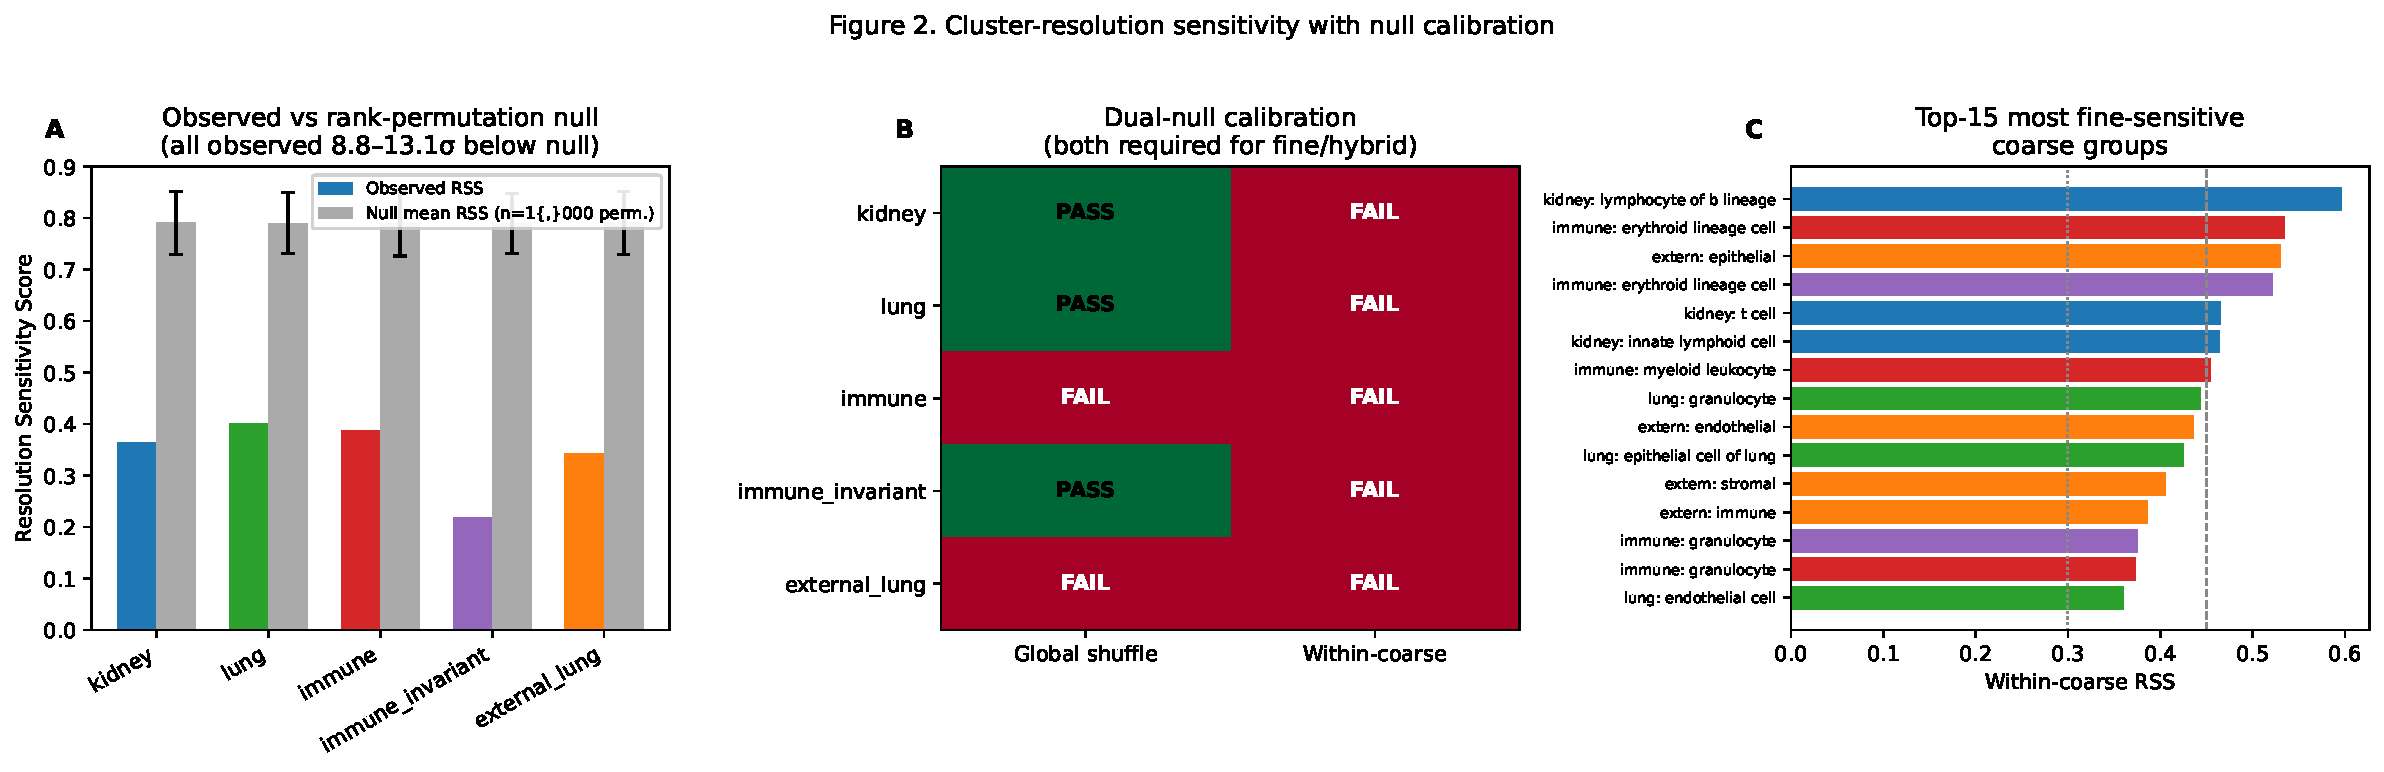
\includegraphics[width=\textwidth,height=0.82\textheight,keepaspectratio]{figures/fig2_resolution.pdf}
%DIFDELCMD < \caption{\textbf{Cluster-resolution sensitivity and dual-null calibration.}
%DIFDELCMD < (A)~Resolution Sensitivity Score across five cohorts with base recommendation thresholds.
%DIFDELCMD < (B)~Dual-null calibration results: global-shuffle and within-coarse constrained-shuffle
%DIFDELCMD < pass/fail for each cohort, with final calibrated recommendation.}
%DIFDELCMD < \label{fig:resolution}
%DIFDELCMD < \end{figure}
%DIFDELCMD < %%%
\DIFdelend \DIFaddbegin \begin{figure*}[ht]
\centering
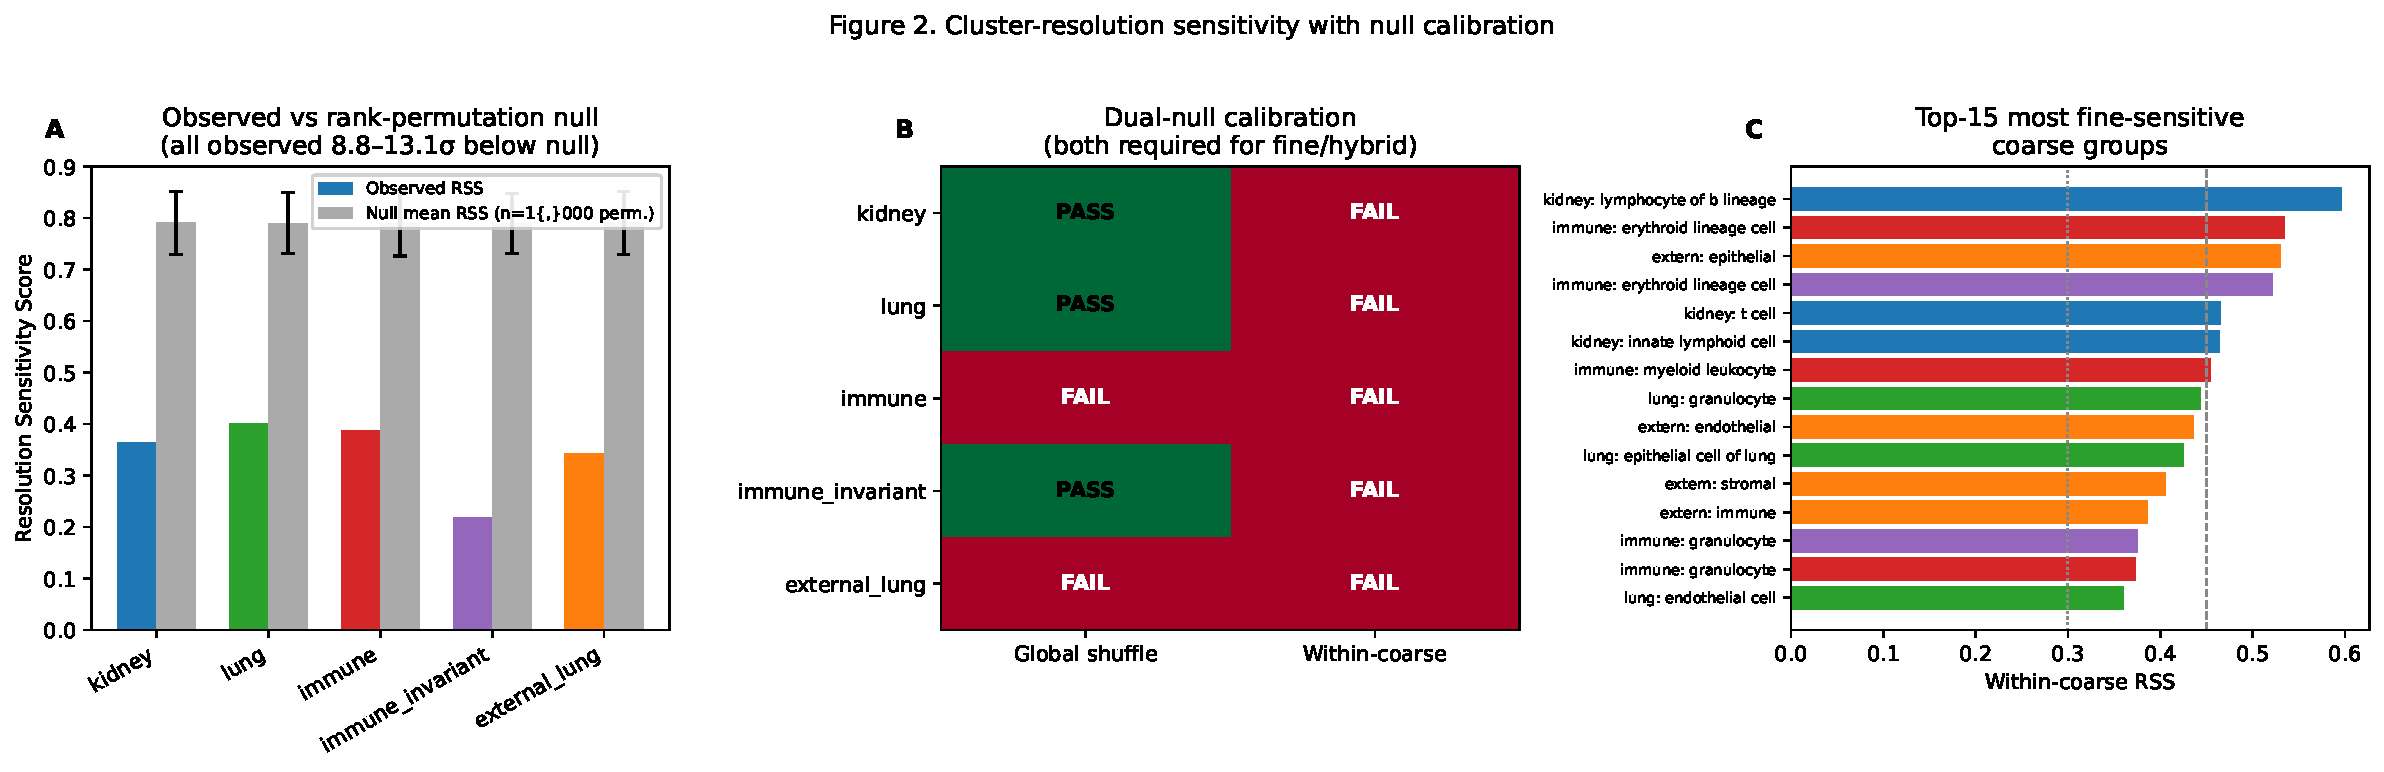
\includegraphics[width=\textwidth,height=0.82\textheight,keepaspectratio]{figures/fig2_resolution.pdf}
\caption{\textbf{Cluster-resolution sensitivity and dual-null calibration.}
(A)~Observed bounded-drift Resolution Sensitivity Score (coloured bars)
versus the rank-permutation null mean and 5th--95th percentile (grey
error bars) for each Tabula Sapiens cohort; every observed value sits
8.8--13.1 standard deviations below the null. (B)~Dual-null pass/fail
heatmap: only kidney, lung, and immune-invariant clear the global
cell-label shuffle; no cohort clears the within-coarse constrained
shuffle. (C)~Top-15 most fine-sensitive coarse groups by within-coarse
RSS; dotted lines mark the base-RSS ``fine'' (0.30) and ``hybrid''
(0.45) thresholds. Colour encodes the cohort of origin.}
\label{fig:resolution}
\end{figure*}
\DIFaddend 

\DIFdelbegin %DIFDELCMD < \subsection{Axis~3: Rare cell types exhibit a systematic reliability gap}
%DIFDELCMD < %%%
\DIFdelend \DIFaddbegin \subsection{Axis~3: Rare cell types exhibit a reliability gap that is
robust to 5{,}880 threshold combinations}
\DIFaddend 

\DIFdelbegin \DIFdel{A natural concern in GRN inference is whether regulatory }\DIFdelend \DIFaddbegin \DIFadd{Are }\DIFaddend edges inferred from rare cell types \DIFdelbegin \DIFdel{(those with few cells in the dataset) are }\DIFdelend as trustworthy as \DIFdelbegin \DIFdel{edges }\DIFdelend \DIFaddbegin \DIFadd{those }\DIFaddend from
abundant types\DIFdelbegin \DIFdel{. }\DIFdelend \DIFaddbegin \DIFadd{? }\DIFaddend Across 88 cell types in \DIFdelbegin \DIFdel{four datasets, the answer depends on which metric is
examined. On a global level, rare types
were not significantly worse at reproducing the
}\DIFdelend \DIFaddbegin \DIFadd{the four adaptive-panel
datasets (three Tabula Sapiens tissues plus external lung), rare types
match abundant types on }\DIFaddend overall rank ordering \DIFdelbegin \DIFdel{across bootstrap replicates (Spearman rank stability: }\DIFdelend \DIFaddbegin \DIFadd{(Spearman }\DIFaddend 0.884 \DIFdelbegin \DIFdel{for
rare versus }\DIFdelend \DIFaddbegin \DIFadd{rare vs
}\DIFaddend 0.851 \DIFdelbegin \DIFdel{for }\DIFdelend abundant, $p = 0.835$) \DIFdelbegin \DIFdel{. This initially reassuring finding masks a
more serious problem: when we looked at whether the
same specific edges appear in the
}\DIFdelend \DIFaddbegin \DIFadd{but are significantly worse on the
decision-relevant }\DIFaddend top-$k$ \DIFdelbegin \DIFdel{list across replicates (a more decision-relevant question, since practitioners
act on specific top-ranked edges), rare types performed significantly worse. Top-$k$
Jaccard was }\DIFdelend \DIFaddbegin \DIFadd{overlap measures: Jaccard }\DIFaddend 0.625 \DIFdelbegin \DIFdel{for rare types versus }\DIFdelend \DIFaddbegin \DIFadd{vs }\DIFaddend 0.731
\DIFdelbegin \DIFdel{for abundant types
}\DIFdelend ($p = 4.1 \times 10^{-3}$), null-separation AUC \DIFdelbegin \DIFdel{was }\DIFdelend 0.520 \DIFdelbegin \DIFdel{versus }\DIFdelend \DIFaddbegin \DIFadd{vs }\DIFaddend 0.620
($p = 5.3 \times 10^{-8}$), \DIFdelbegin \DIFdel{and the null-tail gap (measuring how well genuine signal
separates from noise) was negative for rare types (}\DIFdelend \DIFaddbegin \DIFadd{tail gap }\DIFaddend $-0.062$ \DIFdelbegin \DIFdel{) versus positive for
abundant types ($0.082$; }\DIFdelend \DIFaddbegin \DIFadd{vs $+0.082$
(}\DIFaddend $p = 1.5 \times 10^{-7}$). \DIFdelbegin \DIFdel{In plain terms, edges from rare
cell types are not only less reproducible at the specific-edge level, but their top
scores often fail to separate from what a null model would produce.
}%DIFDELCMD < 

%DIFDELCMD < %%%
\DIFdel{The practical consequence was stark: applying a multi-criteria }\DIFdelend \DIFaddbegin \DIFadd{Under the pre-registered }\DIFaddend reliability gate
(\DIFdelbegin \DIFdel{requiring
adequate stability }\DIFdelend \DIFaddbegin \DIFadd{stability $\geq 0.75$, Jaccard $\geq 0.35$, primary AUC $\geq 0.65$}\DIFaddend ,
\DIFdelbegin \DIFdel{Jaccard, null-separation AUC , }\DIFdelend positive tail gap, \DIFdelbegin \DIFdel{and a minimum of 80
cells), none of the 22 rare cell types passed, compared to 4 of 22 abundant types
}\DIFdelend \DIFaddbegin \DIFadd{cell count $\geq 80$), }\textbf{\DIFadd{0 of 22 rare cell
types pass versus 4 of 22 abundant types}}
\DIFaddend (Figure~\ref{fig:rare}A--B)\DIFdelbegin \DIFdel{. Even under a conservative }\DIFdelend \DIFaddbegin \DIFadd{; under a }\DIFaddend dual-null formulation (\DIFdelbegin \DIFdel{taking the }\DIFdelend minimum
AUC across \DIFdelbegin \DIFdel{both }\DIFdelend cell-permutation and gene-shuffle \DIFdelbegin \DIFdel{null models}\DIFdelend \DIFaddbegin \DIFadd{nulls}\DIFaddend ), the \DIFdelbegin \DIFdel{rare--abundant gap
attenuated but remained }\DIFdelend \DIFaddbegin \DIFadd{gap
attenuates but stays }\DIFaddend significant (AUC gap 0.018,
$p = 6.8 \times 10^{-4}$).

\DIFdelbegin \DIFdel{We investigated whether the gene panel used for edge scoring might explain this gap. A shared-panel sensitivity analysis (fixing 36 }\DIFdelend \DIFaddbegin \DIFadd{A 5}{\DIFadd{,}}\DIFadd{880-point threshold grid (5-D sweep over stability, Jaccard,
AUC, tail gap, and cell count) confirms the headline is not
threshold-driven: the abundant-$>$-rare gap direction holds at
}\emph{\DIFadd{100\%}} \DIFadd{of grid points, the grid-mean gap is $+0.344$ (wider
than $+0.182$ at primary thresholds), and rare pass rate is 0 at
two-thirds of grid points (Supplementary Fig.~S4). Switching to a
shared 36-edge }\DIFaddend TRRUST-intersected \DIFdelbegin \DIFdel{edges across all datasets) showed heterogeneous agreement with the adaptive-panel results: strong concordance in
}\DIFdelend \DIFaddbegin \DIFadd{panel preserves the gap direction
on }\DIFaddend immune and kidney (Spearman 0.93 and 0.87 for null-AUC ordering)
but \DIFdelbegin \DIFdel{weak in lung (Spearman }\DIFdelend \DIFaddbegin \DIFadd{not lung (}\DIFaddend 0.09)\DIFdelbegin \DIFdel{, indicating that panel-construction choices explain part but not all of
the rare-type deficit}\DIFdelend \DIFaddbegin \DIFadd{; the shared ``primary'' panel
(DoRothEA A/B $\cap$ TRRUST) on all five Tabula Sapiens cohorts also
preserves it (0\% rare / 5.9\% intermediate / 9.1\% abundant;
Supplementary Table~S3)}\DIFaddend . Minimum reliable cell-size estimates \DIFdelbegin \DIFdel{ranged }\DIFdelend \DIFaddbegin \DIFadd{under
the adaptive-panel pipeline range }\DIFaddend from 287 \DIFdelbegin \DIFdel{for external lung(model-based extrapolation}\DIFdelend \DIFaddbegin \DIFadd{(external lung,
extrapolated}\DIFaddend ) to 16{,}486 \DIFdelbegin \DIFdel{for lung (empirical reliable minimum), underscoring that }\DIFdelend \DIFaddbegin \DIFadd{(lung, empirical), so }\DIFaddend some tissues require
very large cell-type samples before mechanistic edges clear \DIFdelbegin \DIFdel{reliability thresholds }\DIFdelend \DIFaddbegin \DIFadd{the
reliability gate }\DIFaddend (Figure~\ref{fig:rare}C).

\DIFdelbegin %DIFDELCMD < \begin{figure}[ht]
%DIFDELCMD < \centering
%DIFDELCMD < 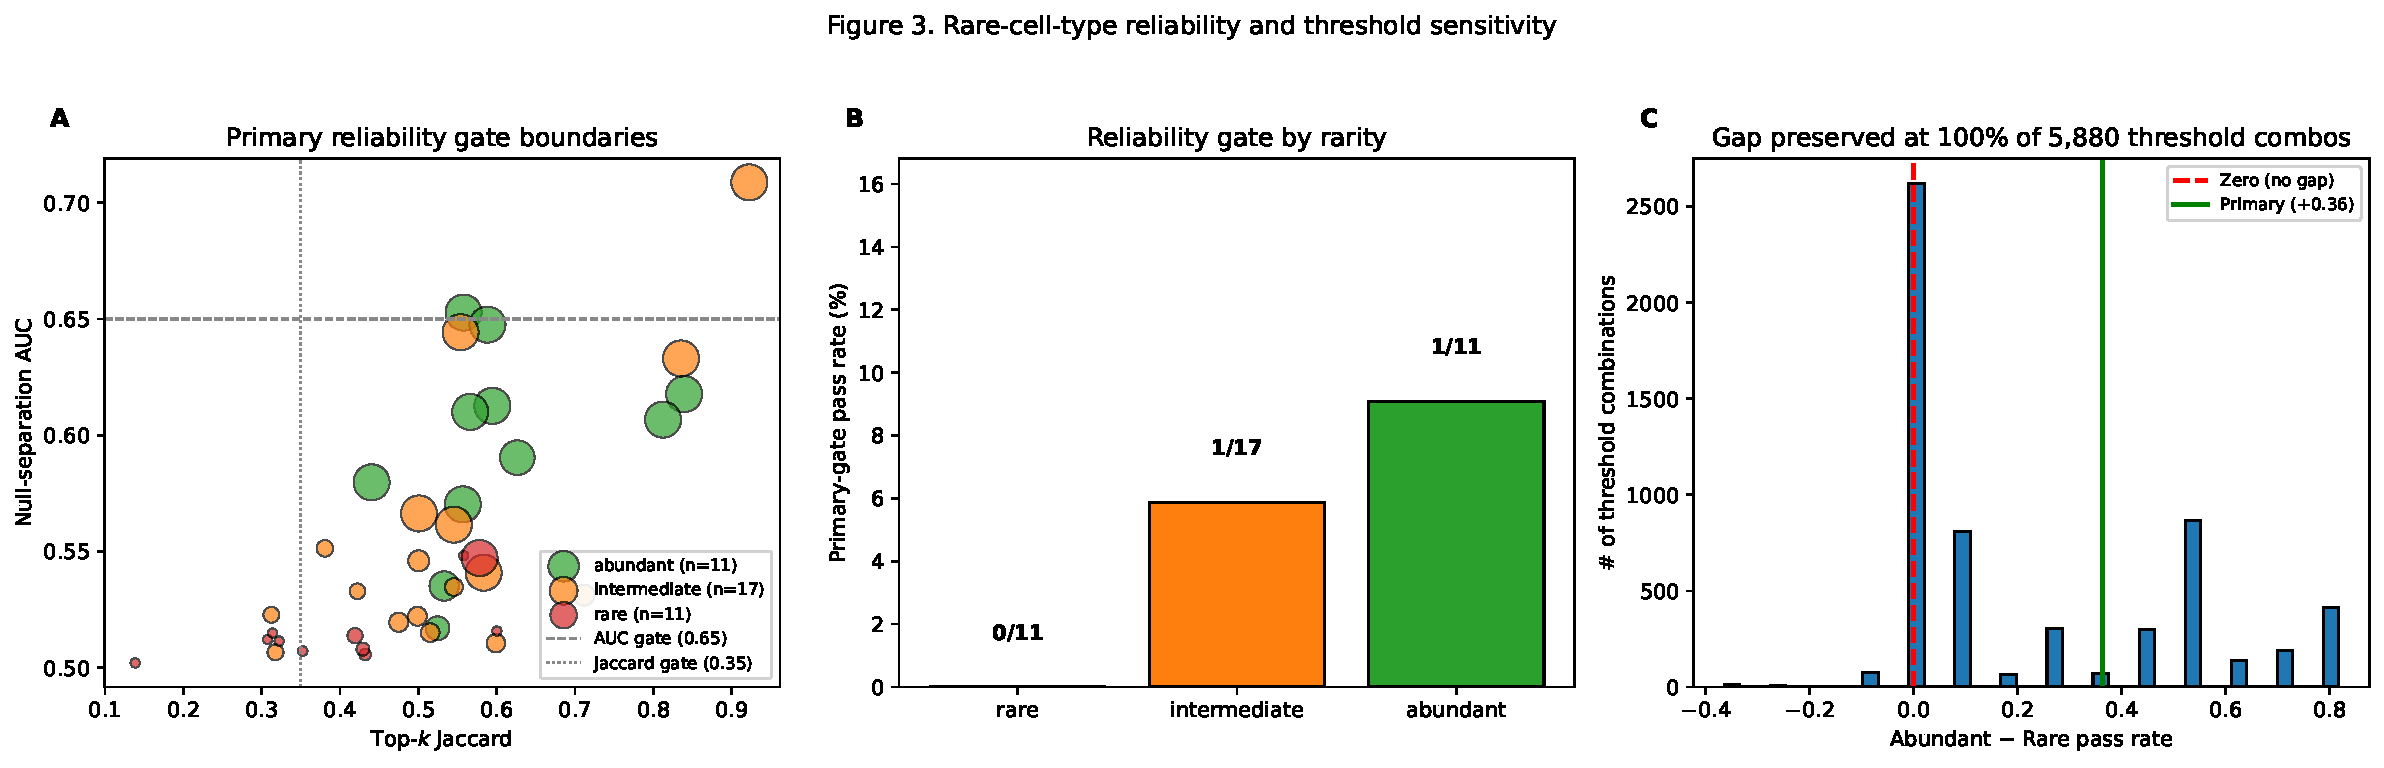
\includegraphics[width=\textwidth,height=0.82\textheight,keepaspectratio]{figures/fig3_rare.pdf}
%DIFDELCMD < \caption{\textbf{Rare-cell-type reliability stress test.}
%DIFDELCMD < (A)~Null-separation AUC and top-$k$ Jaccard as functions of cell count, colored by
%DIFDELCMD < rarity group. (B)~Reliability-gate pass rates: 0\% rare versus 18\% abundant.
%DIFDELCMD < (C)~Minimum reliable cell-size estimates by dataset.}
%DIFDELCMD < \label{fig:rare}
%DIFDELCMD < \end{figure}
%DIFDELCMD < %%%
\DIFdelend \DIFaddbegin \paragraph{Disease-cohort validation.}
\DIFadd{Delorey COVID lung (116}{\DIFadd{,}}\DIFadd{313 cells, 27 donors) presents a
qualitatively different failure mode: across nine coarse compartments,
rank stability is high (Spearman 0.85--0.89) and Jaccard reasonable
(0.53--0.63), but null-separation AUC is uniformly weak (0.50--0.64),
so }\textbf{\DIFadd{no cell type passes the gate in any rarity class}} \DIFadd{(0 of 3
each). Disease-driven shared expression programmes (COVID-induced
myeloid / fibroblast remodelling) plausibly compress the
observed-vs-null gap; the gate was calibrated on Tabula Sapiens and
may need disease-specific recalibration for heavily perturbed tissues.
}\DIFaddend 

\DIFdelbegin %DIFDELCMD < \subsection{Axis~4: Donor generalization requires 6--8 donors and is partly composition-mediated}
%DIFDELCMD < %%%
\DIFdelend \DIFaddbegin \begin{figure*}[ht]
\centering
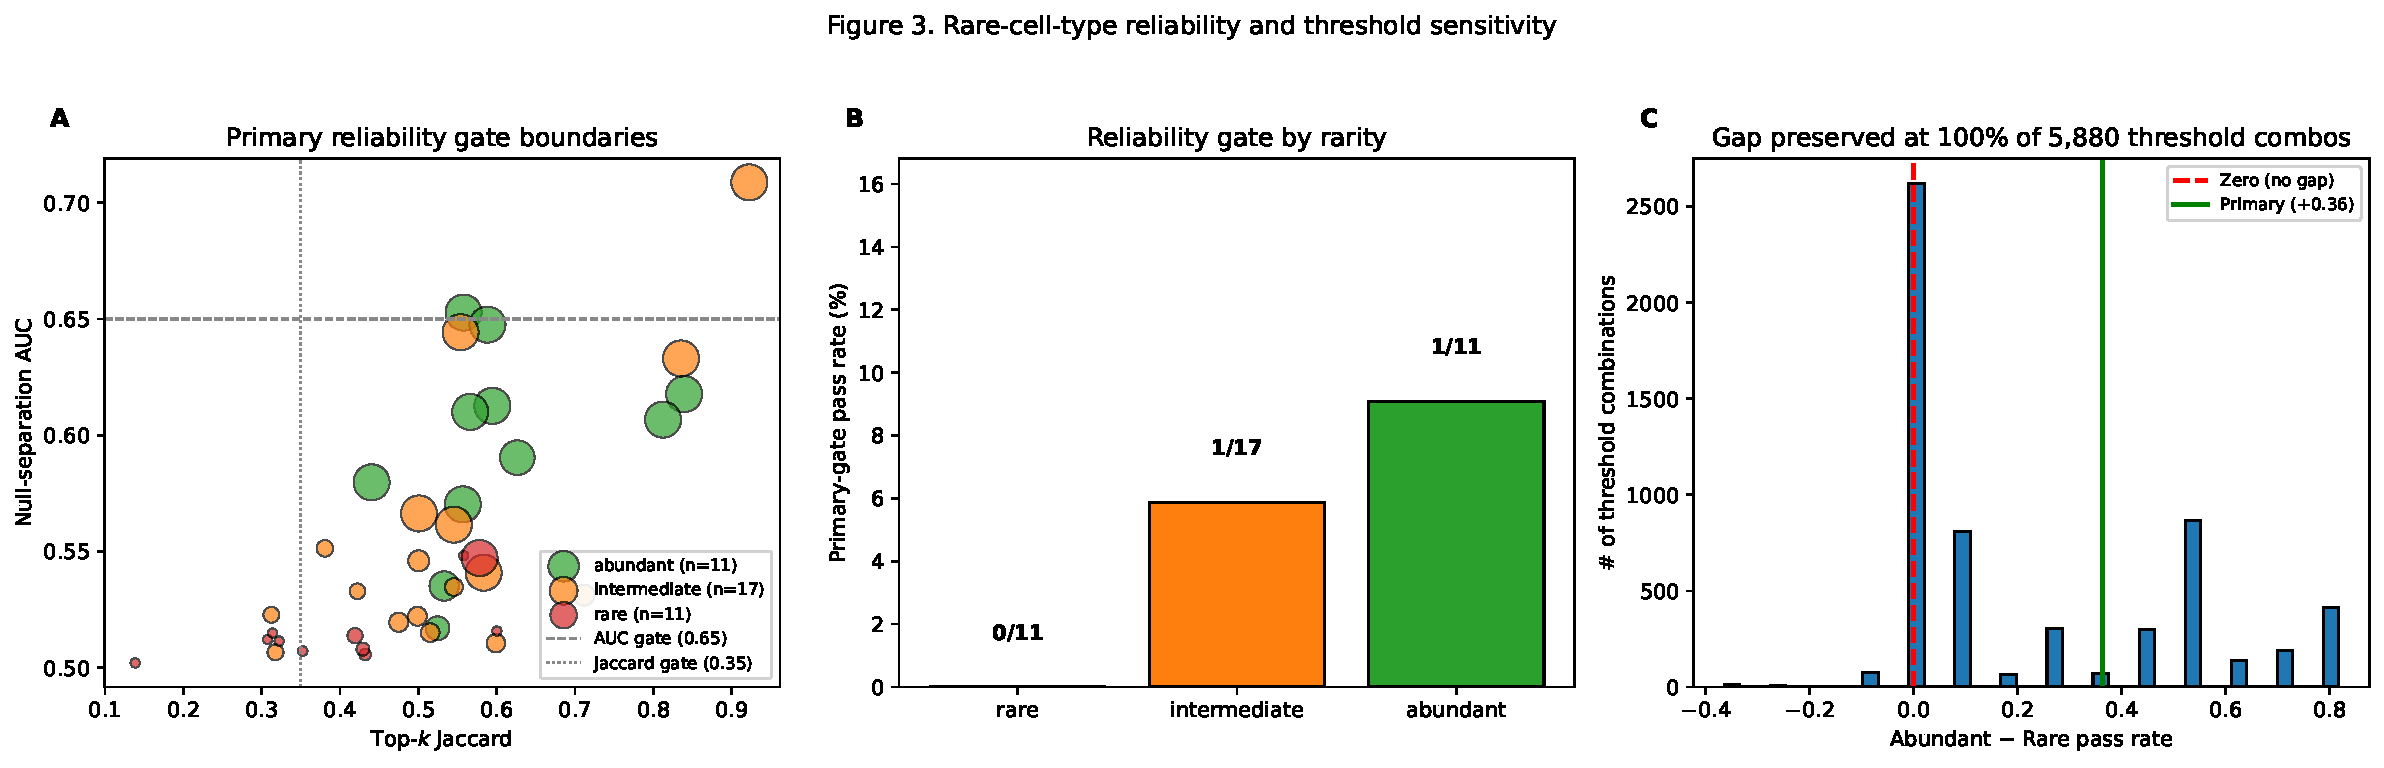
\includegraphics[width=\textwidth,height=0.82\textheight,keepaspectratio]{figures/fig3_rare.pdf}
\caption{\textbf{Rare-cell-type reliability and threshold sensitivity.}
(A)~Scatter of null-separation AUC versus top-$k$ Jaccard for every
eligible cell type, coloured by within-dataset rarity group (rare
/ intermediate / abundant). Marker size scales with cell count.
Dashed grey lines mark the primary-gate thresholds
(AUC $\geq 0.65$, Jaccard $\geq 0.35$); points in the upper-right
quadrant are candidates for passing. (B)~Primary-gate pass rates by
rarity on the shared ``primary'' panel (fragility package output);
numerators/denominators shown above each bar. (C)~Histogram of the
abundant-minus-rare pass-rate gap across all 5{,}880 threshold
combinations on the five-dimensional grid; the primary-threshold gap
is marked in green and zero (no gap) in red. The gap direction is
preserved at 100\% of grid points.}
\label{fig:rare}
\end{figure*}
\DIFaddend 

\DIFdelbegin \DIFdel{This axis asks: if a GRN is inferred from one set of donors,will the same edges be
prioritized when applied to a
completely different set of donors from the same tissue?
This question is central to generalizability,
since most single-cell atlases pool
multiple individuals, and differences in donor composition (genetics, health status,
sample quality)can drive variation that is biological but not regulatory. }%DIFDELCMD < 

%DIFDELCMD < %%%
\DIFdel{Under the corrected }\DIFdelend \DIFaddbegin \subsection{Axis~4: Donor generalization improves monotonically; the
required donor count depends on cells-per-donor balancing}

\DIFadd{Under the }\DIFaddend fixed-holdout protocol (\DIFdelbegin \DIFdel{where }\DIFdelend two holdout donors \DIFdelbegin \DIFdel{are kept constantas the training set grows}\DIFdelend \DIFaddbegin \DIFadd{held constant}\DIFaddend ),
immune-tissue transfer \DIFdelbegin \DIFdel{improved monotonically }\DIFdelend \DIFaddbegin \DIFadd{improves monotonically with training-donor count.
At 300 cells/donor in the 20k-cell immune subset, Spearman $\rho$ rises
0.568 $\to$ 0.683 }\DIFaddend from 2 to 10 training donors \DIFdelbegin \DIFdel{(Spearman 0.568 $\to$ 0.683; }\DIFdelend \DIFaddbegin \DIFadd{and }\DIFaddend top-100 overlap
\DIFaddbegin \DIFadd{rises }\DIFaddend 0.445 $\to$ 0.540 \DIFdelbegin \DIFdel{;
}\DIFdelend \DIFaddbegin \DIFadd{(}\DIFaddend Figure~\ref{fig:donor}A). \DIFdelbegin \DIFdel{This monotonic curve eliminated an apparent interior optimum
that had appeared in the initial complementary-split design, where adding more training
donors mechanically shrank the holdout set and artificially inflated transfer estimates
by $+0.080$ Spearman on average.
}%DIFDELCMD < 

%DIFDELCMD < %%%
\DIFdel{Including donors from the long tail of the cohort (expanding from the top-12 }\DIFdelend \DIFaddbegin \DIFadd{Expanding }\DIFaddend to the
top-20 donors \DIFdelbegin \DIFdel{by cell count) lowered }\DIFdelend \DIFaddbegin \DIFadd{(long-tail inclusion) lowers }\DIFaddend all transfer metrics
(\DIFdelbegin \DIFdel{Spearman 0.627 }\DIFdelend \DIFaddbegin \DIFadd{$\rho = 0.627$ }\DIFaddend at 16 \DIFdelbegin \DIFdel{training
donors versus }\DIFdelend \DIFaddbegin \DIFadd{donors vs }\DIFaddend 0.683 at 10 \DIFdelbegin \DIFdel{training donors under }\DIFdelend \DIFaddbegin \DIFadd{in }\DIFaddend the top-12 \DIFdelbegin \DIFdel{protocol),
revealing that evaluations restricted to the highest-quality donors give }\DIFdelend \DIFaddbegin \DIFadd{panel),
showing that high-quality-donor restrictions paint }\DIFaddend an optimistic picture\DIFdelbegin \DIFdel{of how
rankings will generalize in broader deployment settings.
Based on these curves, the
}\DIFdelend \DIFaddbegin \DIFadd{.
The }\DIFaddend 90\%-of-best criterion recommends \DIFdelbegin \DIFdel{a minimum of }\DIFdelend \textbf{6 training donors}\DIFdelbegin \DIFdel{, while the
more conservative }\DIFdelend \DIFaddbegin \DIFadd{; the
}\DIFaddend 95\%-of-best criterion recommends \textbf{8\DIFdelbegin \DIFdel{donors}\DIFdelend }. \DIFaddbegin \DIFadd{Under looser balancing
(200 cells/donor, 13 eligible donors), the curve shifts and 90\%-of-best
is met at 2 donors --- the requirement is therefore
}\emph{\DIFadd{cells-per-donor dependent}}\DIFadd{, and the cells-per-donor policy must
be pre-registered.
}\DIFaddend 

\DIFdelbegin \DIFdel{A follow-up analysis controlled for cell-type composition by matching donors on broad
cell classes }\DIFdelend \DIFaddbegin \DIFadd{Composition matching }\DIFaddend (3 shared \DIFaddbegin \DIFadd{cell }\DIFaddend classes, 62 cells\DIFdelbegin \DIFdel{per donor) . Composition-matched transfer was
}\DIFdelend \DIFaddbegin \DIFadd{/donor) lowers
transfer by }\DIFaddend 16.3\% \DIFdelbegin \DIFdel{lower for Spearman correlation }\DIFdelend \DIFaddbegin \DIFadd{on Spearman }\DIFaddend (0.707 $\to$ 0.591) and 10.7\% \DIFdelbegin \DIFdel{lower for }\DIFdelend \DIFaddbegin \DIFadd{on
}\DIFaddend top-100 overlap (0.610 $\to$ 0.545; Figure~\ref{fig:donor}B)\DIFdelbegin \DIFdel{, confirming that }\DIFdelend \DIFaddbegin \DIFadd{: }\DIFaddend a
substantial fraction of apparent donor \DIFdelbegin \DIFdel{generalization }\DIFdelend \DIFaddbegin \DIFadd{generalisation }\DIFaddend reflects
shared cell-type composition\DIFdelbegin \DIFdel{rather
than genuine regulatory consistency across individuals. Nevertheless, even }\DIFdelend \DIFaddbegin \DIFadd{. Even }\DIFaddend under this strictest protocol \DIFdelbegin \DIFdel{, }\DIFdelend the
above-null signal \DIFdelbegin \DIFdel{remained }\DIFdelend \DIFaddbegin \DIFadd{remains }\DIFaddend large (lift@100 of 37.8--44.3$\times$\DIFdelbegin \DIFdel{over chance}\DIFdelend ),
indicating \DIFdelbegin \DIFdel{that }\DIFdelend real cross-donor regulatory signal \DIFdelbegin \DIFdel{persists beyond what compositiondifferences alone can explain}\DIFdelend \DIFaddbegin \DIFadd{beyond composition}\DIFaddend .

\DIFdelbegin %DIFDELCMD < \begin{figure}[ht]
%DIFDELCMD < \centering
%DIFDELCMD < 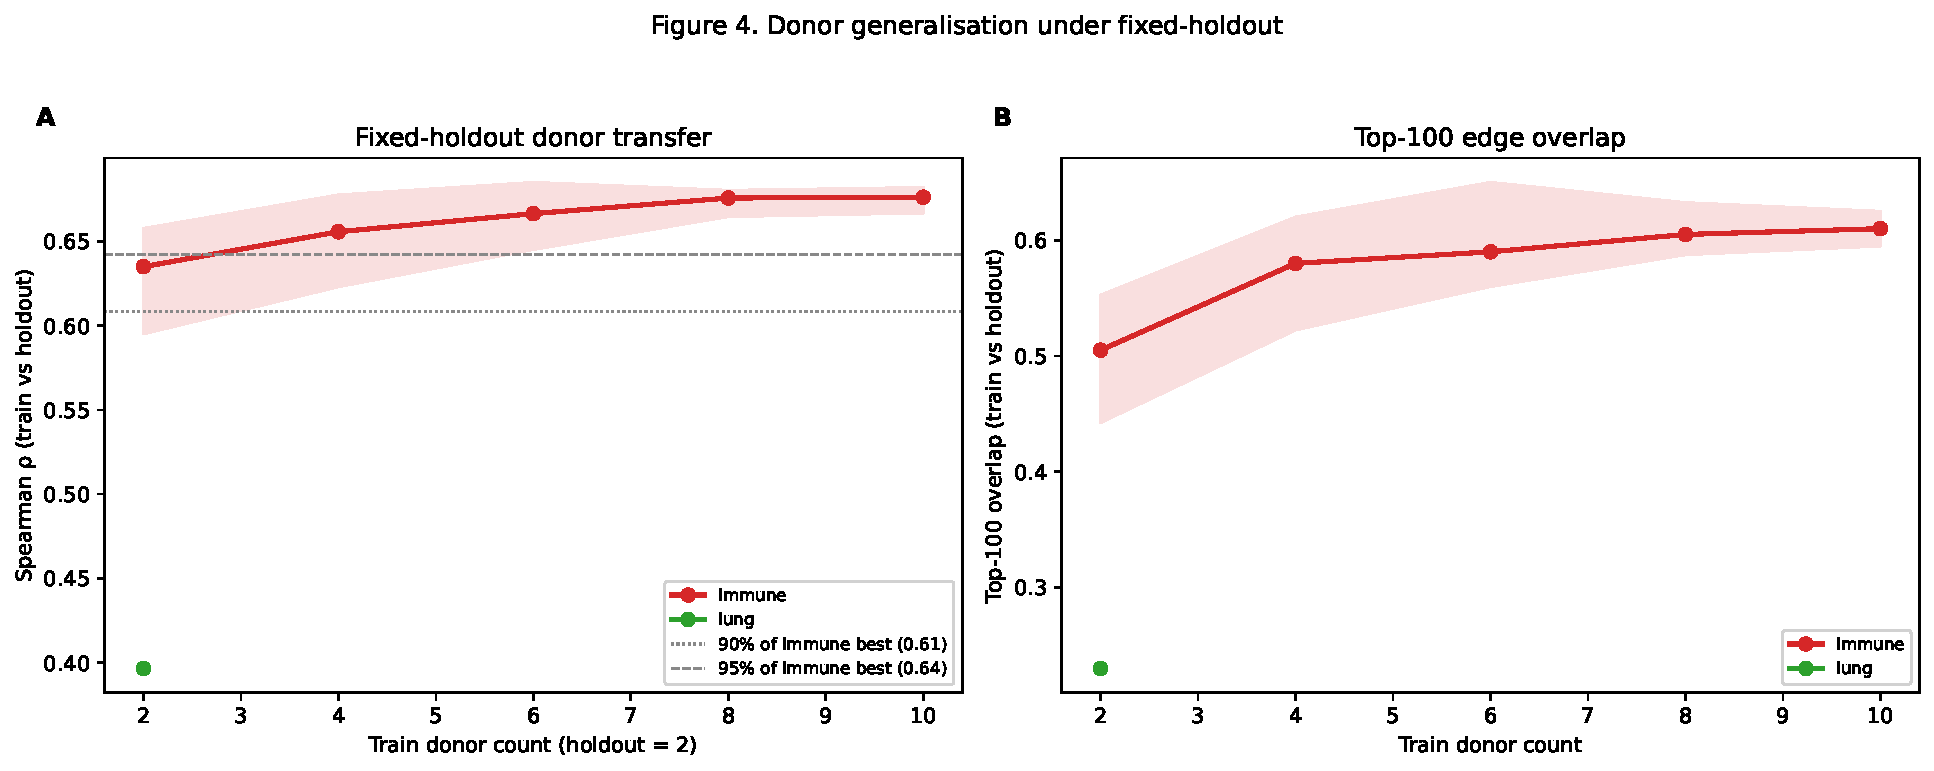
\includegraphics[width=\textwidth]{figures/fig4_donor.pdf}
%DIFDELCMD < \caption{\textbf{Donor generalization under fixed-holdout and composition control.}
%DIFDELCMD < (A)~Immune transfer curves under fixed-holdout (holdout$= 2$) for top-12 and top-20
%DIFDELCMD < donor panels. (B)~Composition-matched versus unmatched transfer in the top-8 panel.
%DIFDELCMD < Error bands show interquartile range over 30--40 sampled splits.}
%DIFDELCMD < \label{fig:donor}
%DIFDELCMD < \end{figure}
%DIFDELCMD < %%%
\DIFdelend \DIFaddbegin \begin{figure*}[ht]
\centering
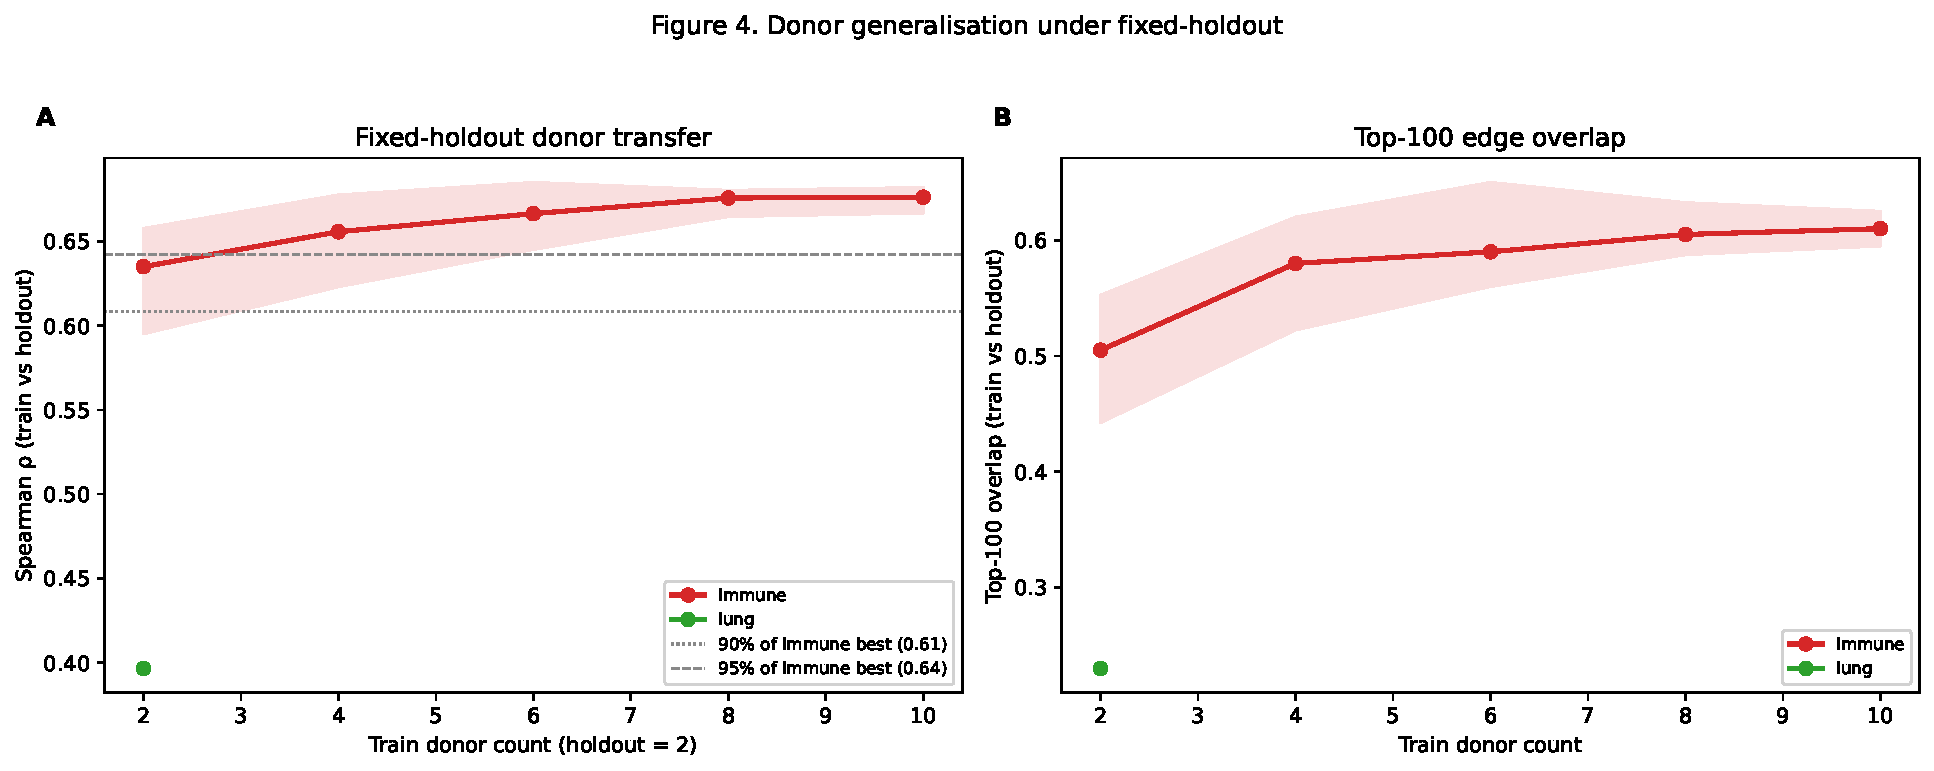
\includegraphics[width=\textwidth]{figures/fig4_donor.pdf}
\caption{\textbf{Donor generalization under fixed-holdout and composition control.}
(A)~Immune transfer curves under fixed-holdout (holdout$= 2$) for top-12 and top-20
donor panels. (B)~Composition-matched versus unmatched transfer in the top-8 panel.
Error bands show interquartile range over 30--40 sampled splits.}
\label{fig:donor}
\end{figure*}
\DIFaddend 

\DIFdelbegin %DIFDELCMD < \subsection{Axis~5: Integration reorders rankings substantially but does not improve perturbation-grounded validity}
%DIFDELCMD < %%%
\DIFdelend \DIFaddbegin \subsection{Axis~5: Integration method choice reorders rankings
substantially and does not improve perturbation-grounded validity}
\DIFaddend 

\DIFdelbegin \DIFdel{Batch correction is a standard step in multi-sample single-cell analysis, but its
effect on downstream GRN edge rankings is rarely examined. Here, applying Harmony integration produced }\DIFdelend \DIFaddbegin \DIFadd{Harmony integration produces }\DIFaddend moderate-to-large rank perturbations \DIFdelbegin \DIFdel{across }\DIFdelend \DIFaddbegin \DIFadd{on
}\DIFaddend all three tissues\DIFdelbegin \DIFdel{:
Spearman correlation between corrected and uncorrected rankings ranged from }\DIFdelend \DIFaddbegin \DIFadd{. On the full HVG-pair universe (unconstrained),
Spearman corrected-vs-uncorrected ranges }\DIFaddend 0.757\DIFdelbegin \DIFdel{to
0.823, }\DIFdelend \DIFaddbegin \DIFadd{--0.823 with }\DIFaddend sign-flip
rates \DIFdelbegin \DIFdel{(edges whose inferred direction of regulation reversed)ranged
from 8.1\%to 12.7\%, and only 55--69\% of the }\DIFdelend \DIFaddbegin \DIFadd{8.1--12.7\%. Panel-restricted (hematopoiesis $76 \times 108$):
}\DIFaddend top-500 \DIFdelbegin \DIFdel{edges were shared between the
two conditions }\DIFdelend \DIFaddbegin \DIFadd{overlap 65--71\%, top-1}{\DIFadd{,}}\DIFadd{000 overlap 72--75\%, i.e.\
29--35\% top-500 displacement }\DIFaddend (Figure~\ref{fig:integration}A) \DIFdelbegin \DIFdel{. In concrete terms, }\DIFdelend \DIFaddbegin \DIFadd{---
}\DIFaddend roughly a third of \DIFdelbegin \DIFdel{the edges an analyst would prioritize }\DIFdelend \DIFaddbegin \DIFadd{prioritised edges }\DIFaddend change depending on whether
batch correction is applied\DIFaddbegin \DIFadd{. Yet rankings stay highly non-random:
bounded-drift RSS between baseline and Harmony-integrated lists is
0.26--0.30 across the eight (tissue $\times$ batch-key) combinations
vs null mean $\approx 0.72$ ($|z| \geq 37$; empirical $p$ at floor).
}

\paragraph{Integration method matters.}
\DIFadd{A cross-method comparison (Harmony vs scVI vs Scanorama, same
cells, same panel, same random seed) reveals that method choice is
not neutral (Table~\ref{tab:integration_methods}). Three regimes emerge:
}

\begin{itemize}
\item \textbf{\DIFadd{Harmony}} \DIFadd{preserves rankings reasonably well across all
      three tissues (Spearman 0.63--0.87}\DIFaddend , \DIFdelbegin \DIFdel{which raises the question of
      whether the corrected rankings are actually better.
}\DIFdelend \DIFaddbegin \DIFadd{top-1}{\DIFadd{,}}\DIFadd{000 overlap
      0.65--0.87, sign-flip 6--17\%).
}\item \textbf{\DIFadd{scVI}} \DIFadd{sits in the middle: Spearman 0.36--0.57, top-1}{\DIFadd{,}}\DIFadd{000
      overlap 0.48--0.74, sign-flip 18--30\%. Roughly a quarter of
      edges change sign compared to the uncorrected baseline.
}\item \textbf{\DIFadd{Scanorama}} \DIFadd{produces near-random rankings on kidney and
      lung (Spearman $\approx 0$, top-1}{\DIFadd{,}}\DIFadd{000 overlap 0.11--0.14,
      sign-flip 44--47\%; RSS at the rank-permutation null mean of
      $\approx 0.72$) and weakly correlated rankings on immune
      (Spearman 0.10, top-1}{\DIFadd{,}}\DIFadd{000 overlap 0.62, sign-flip 26\%).
}\end{itemize}
\DIFaddend 

\DIFdelbegin \DIFdel{To address this, we evaluated whether Harmony-corrected rankings improve agreement with
curated reference databases.
At the level of raw }\DIFdelend \DIFaddbegin \DIFadd{In other words, switching integration method on the same data can
cause anywhere from 6\% to 47\% of the top-500 edges to change sign,
and can move the top-1}{\DIFadd{,}}\DIFadd{000 ranking to statistical indistinguishability
from a random rewire of the baseline. Any GRN claim downstream of
integration therefore depends materially on integration-method choice;
we recommend reporting rank-stability metrics against the uncorrected
baseline for every integration tool used.
}

\begin{table*}[ht]
\centering
\caption{Cross-method integration perturbation of edge rankings.
All rows: 1{,}200 cells, hematopoiesis $76 \times 108$ panel,
Pearson scorer, same random seed. Top-1{,}000 overlap below $\sim 0.3$
with RSS at the rank-permutation null mean $\approx 0.72$ indicates
near-random rankings.}
\label{tab:integration_methods}
\small
\begin{tabular}{llrrrrr}
\toprule
\textbf{Dataset} & \textbf{Method} & \textbf{Spearman} &
\textbf{Overlap@500} & \textbf{Overlap@1k} &
\textbf{Sign-flip} & \textbf{RSS@500} \\
\midrule
Kidney & Harmony    &  0.78 & 0.62 & 0.69 & 15\% & 0.38 \\
Kidney & scVI       &  0.57 & 0.42 & 0.51 & 24\% & 0.51 \\
Kidney & Scanorama  & -0.04 & 0.08 & 0.11 & 47\% & 0.76 \\
Lung   & Harmony    &  0.63 & 0.59 & 0.65 & 17\% & 0.42 \\
Lung   & scVI       &  0.36 & 0.42 & 0.48 & 30\% & 0.54 \\
Lung   & Scanorama  & -0.02 & 0.08 & 0.14 & 44\% & 0.77 \\
Immune & Harmony    &  0.87 & 0.81 & 0.87 &  6\% & 0.20 \\
Immune & scVI       &  0.54 & 0.63 & 0.74 & 18\% & 0.37 \\
Immune & Scanorama  &  0.10 & 0.32 & 0.62 & 26\% & 0.60 \\
\bottomrule
\end{tabular}
\end{table*}

\paragraph{Do integrated rankings better recover reference edges?}
\DIFadd{Raw }\DIFaddend precision@500 \DIFdelbegin \DIFdel{, nominal gains appeared
for both }\DIFdelend \DIFaddbegin \DIFadd{shows nominal Harmony gains on }\DIFaddend DoRothEA and TRRUST
\DIFdelbegin \DIFdel{references }\DIFdelend in immune and kidney\DIFdelbegin \DIFdel{tissue. However, after
applying paired swap-based significance tests with Benjamini--Hochberg FDR correction
(a more stringent test that asks whether the gains exceed what pairwise edge reordering
alone could produce), robust improvements were limited to TRRUST in }\DIFdelend \DIFaddbegin \DIFadd{, but paired swap tests with BH-FDR correction
restrict robust improvements to TRRUST on }\DIFaddend immune and kidney
($\Delta$ precision \DIFdelbegin \DIFdel{+0.026 to +0.028}\DIFdelend \DIFaddbegin \DIFadd{$+0.026$ to $+0.028$}\DIFaddend , FDR $< 0.05$;
Figure~\ref{fig:integration}B)\DIFdelbegin \DIFdel{.
DoRothEA- }\DIFdelend \DIFaddbegin \DIFadd{; DoRothEA }\DIFaddend and ChIP-seq--backed gains
\DIFdelbegin \DIFdel{did not survive FDR correction. More importantly,
perturbation validation using experimentally derived regulatory tables from }\DIFdelend \DIFaddbegin \DIFadd{do not survive correction. Perturbation validation against
}\DIFaddend Perturb-seq\DIFdelbegin \DIFdel{data~\mbox{%DIFAUXCMD
\citep{Dixit2016} }\hskip0pt%DIFAUXCMD
showed no significant Harmony improvement: the }\DIFdelend \DIFaddbegin \DIFadd{~\mbox{%DIFAUXCMD
\citep{Dixit2016, Replogle2022} }\hskip0pt%DIFAUXCMD
returns small, negative }\DIFaddend top-500 \DIFdelbegin \DIFdel{perturbation swap
deltas were small and negative }\DIFdelend \DIFaddbegin \DIFadd{swap
deltas }\DIFaddend ($-0.002$ to $-0.004$\DIFdelbegin \DIFdel{; }\DIFdelend \DIFaddbegin \DIFadd{, }\DIFaddend FDR $= 1.0$)\DIFdelbegin \DIFdel{,
meaning that the edges gained by
integration were not }\DIFdelend \DIFaddbegin \DIFadd{: edges }\emph{\DIFadd{gained}} \DIFadd{by
integration are no }\DIFaddend more likely to be experimentally validated than
\DIFdelbegin \DIFdel{the edges lost. }%DIFDELCMD < 

%DIFDELCMD < %%%
\DIFdel{A hyperparameter sweep over the number of principal components
(}\DIFdelend \DIFaddbegin \DIFadd{edges }\emph{\DIFadd{lost}}\DIFadd{. Ranking perturbation does not translate into
biological gain even for the best-behaved integrator. A
}\DIFaddend $n_{\text{pcs}} \in \{30, 50, 80\}$ \DIFdelbegin \DIFdel{) revealed an informative }\DIFdelend \DIFaddbegin \DIFadd{sweep reveals a }\DIFaddend tradeoff: top-500
overlap with \DIFdelbegin \DIFdel{the uncorrected baseline increased monotonically with more }\DIFdelend \DIFaddbegin \DIFadd{baseline rises monotonically with }\DIFaddend PCs (immune
\DIFdelbegin \DIFdel{: 0.590 $\to$
0.736), meaning that higher dimensionality makes integration more conservative and less
disruptive}\DIFdelend \DIFaddbegin \DIFadd{$0.590 \to 0.736$, more conservative integration)}\DIFaddend , but DoRothEA
precision \DIFdelbegin \DIFdel{peaked }\DIFdelend \DIFaddbegin \DIFadd{peaks }\DIFaddend at intermediate PCs \DIFdelbegin \DIFdel{and declined at higher
dimensionality }\DIFdelend (Figure~\ref{fig:integration}C)\DIFdelbegin \DIFdel{. There is thus }\DIFdelend \DIFaddbegin \DIFadd{,
so }\DIFaddend no single setting \DIFdelbegin \DIFdel{that
simultaneously maximizes }\DIFdelend \DIFaddbegin \DIFadd{maximises }\DIFaddend both stability and reference agreement.

\DIFdelbegin %DIFDELCMD < \begin{figure}[ht]
%DIFDELCMD < \centering
%DIFDELCMD < 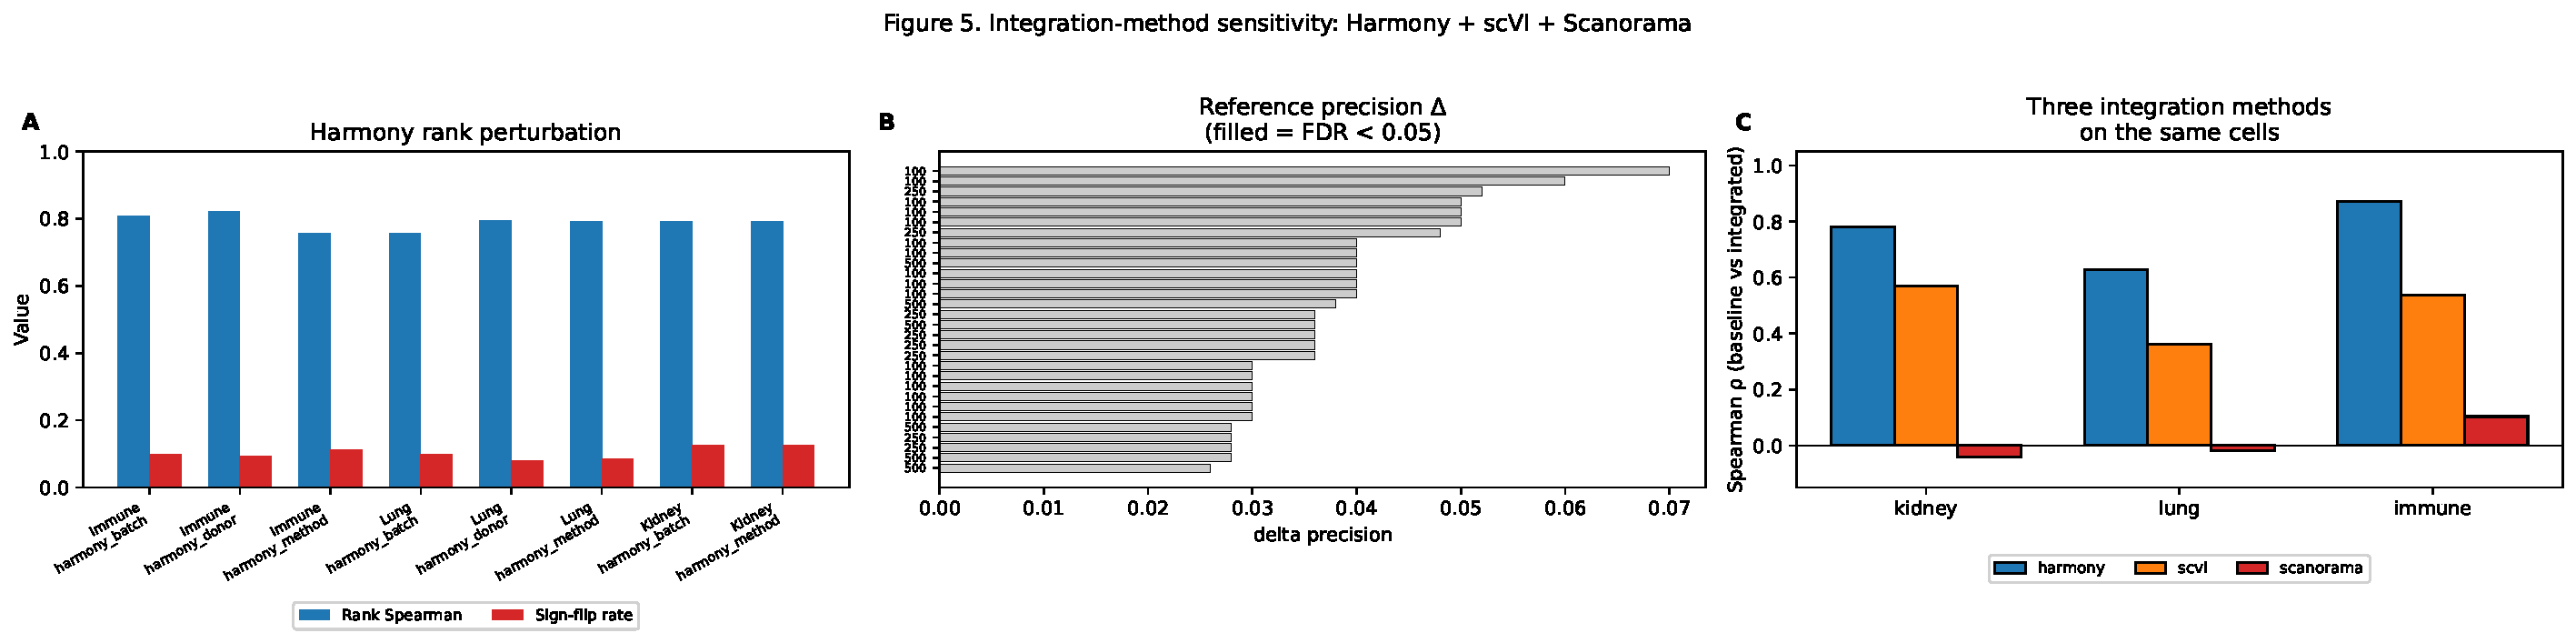
\includegraphics[width=\textwidth,height=0.82\textheight,keepaspectratio]{figures/fig5_integration.pdf}
%DIFDELCMD < \caption{\textbf{Integration-method sensitivity.}
%DIFDELCMD < (A)~Rank Spearman and top-500 overlap for Harmony variants across three tissues.
%DIFDELCMD < (B)~Reference precision@500 deltas with paired swap significance; filled bars indicate
%DIFDELCMD < FDR $< 0.05$. (C)~Harmony hyperparameter sweep: overlap versus DoRothEA precision
%DIFDELCMD < as a function of $n_{\text{pcs}}$.}
%DIFDELCMD < \label{fig:integration}
%DIFDELCMD < \end{figure}
%DIFDELCMD < %%%
\DIFdelend \DIFaddbegin \begin{figure*}[ht]
\centering
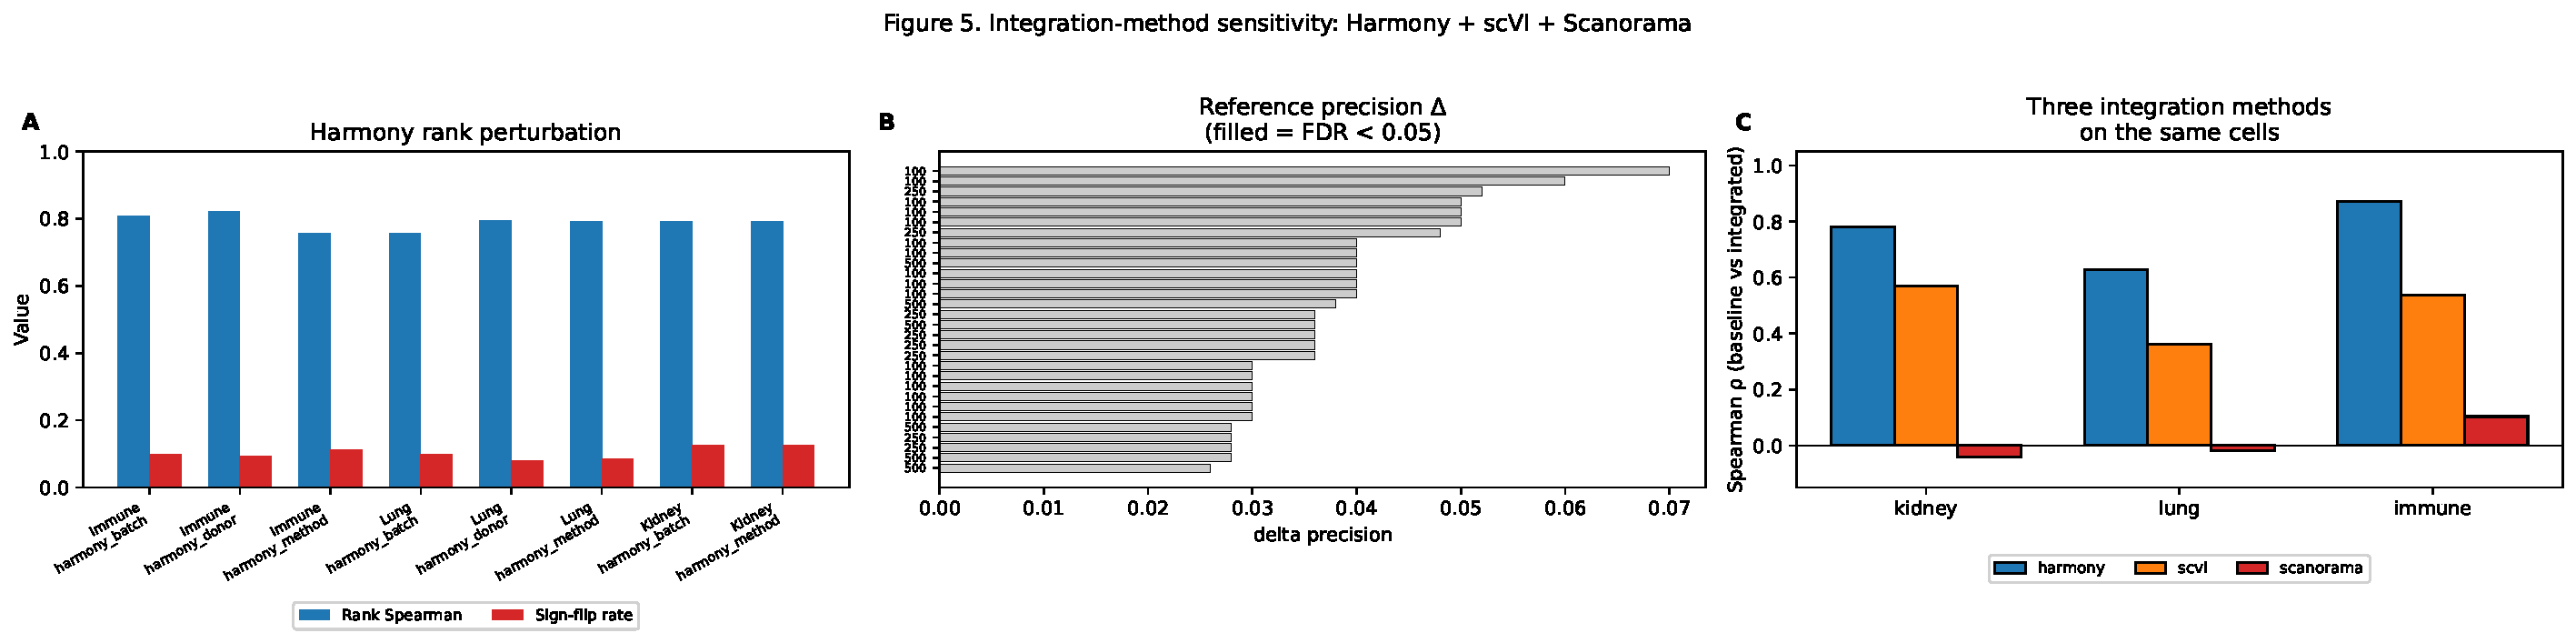
\includegraphics[width=\textwidth,height=0.82\textheight,keepaspectratio]{figures/fig5_integration.pdf}
\caption{\textbf{Integration-method sensitivity.}
(A)~Rank Spearman and sign-flip rate for Harmony variants (tissue
$\times$ batch key combinations) against uncorrected baseline.
(B)~Reference precision@500 deltas for Harmony-integrated vs
uncorrected rankings, with paired swap-based binomial significance
tests (filled bars: FDR $<0.05$ under Benjamini--Hochberg correction;
unfilled: not significant). (C)~Cross-method comparison of three
integration tools: Harmony (blue), scVI (orange), and Scanorama (red),
on 1{,}200 cells from each tissue (Pearson scorer, hematopoiesis
$76 \times 108$ panel). Dashed horizontal line at $\rho = 0$
indicates rank-permutation null.}
\label{fig:integration}
\end{figure*}
\DIFaddend 

\DIFdelbegin %DIFDELCMD < \subsection{Cross-axis fragility synthesis}
%DIFDELCMD < %%%
\DIFdelend \DIFaddbegin \subsection{Scorer divergence: within-scorer fragility does not transfer across scorer families}
\DIFaddend 

\DIFdelbegin \DIFdel{The five axes were designed independently,
but the
fragility they reveal is not
independent.
}\DIFdelend \DIFaddbegin \DIFadd{Scoring the hematopoiesis $76 \times 108$ panel on a shared 800-cell
kidney sample with all five scorers reveals the pairwise agreement
landscape (Table~\ref{tab:scorer_divergence},
Figure~\ref{fig:scorer_divergence}). The two tree-ensemble scorers
(GRNBoost2 and GENIE3) are near-identical (Spearman $\rho = 0.93$,
top-500 Jaccard $= 0.54$); Pearson is moderately correlated with the
tree scorers ($\rho \in [0.52, 0.56]$); mutual information is weakly
correlated with Pearson ($\rho = 0.20$) and unrelated to the tree
scorers ($\rho \leq 0.21$). Most importantly, }\textbf{\DIFadd{scGPT attention
is uncorrelated with every classical scorer}}\DIFadd{: Spearman $\rho$ ranges
$-0.05$ (vs Pearson) to $+0.20$ (vs MI), top-100 Jaccard 0.02--0.06,
and the RSS composite 0.69--0.76 sits at or above the
rank-permutation null mean ($\approx 0.72$). The Axes 1--5
within-scorer fragility analysis is therefore orthogonal to
across-scorer agreement: choosing a stable scorer does not guarantee
another stable scorer will agree with it, and an analyst switching
scorers must re-audit.
}

\begin{figure*}[ht]
\centering
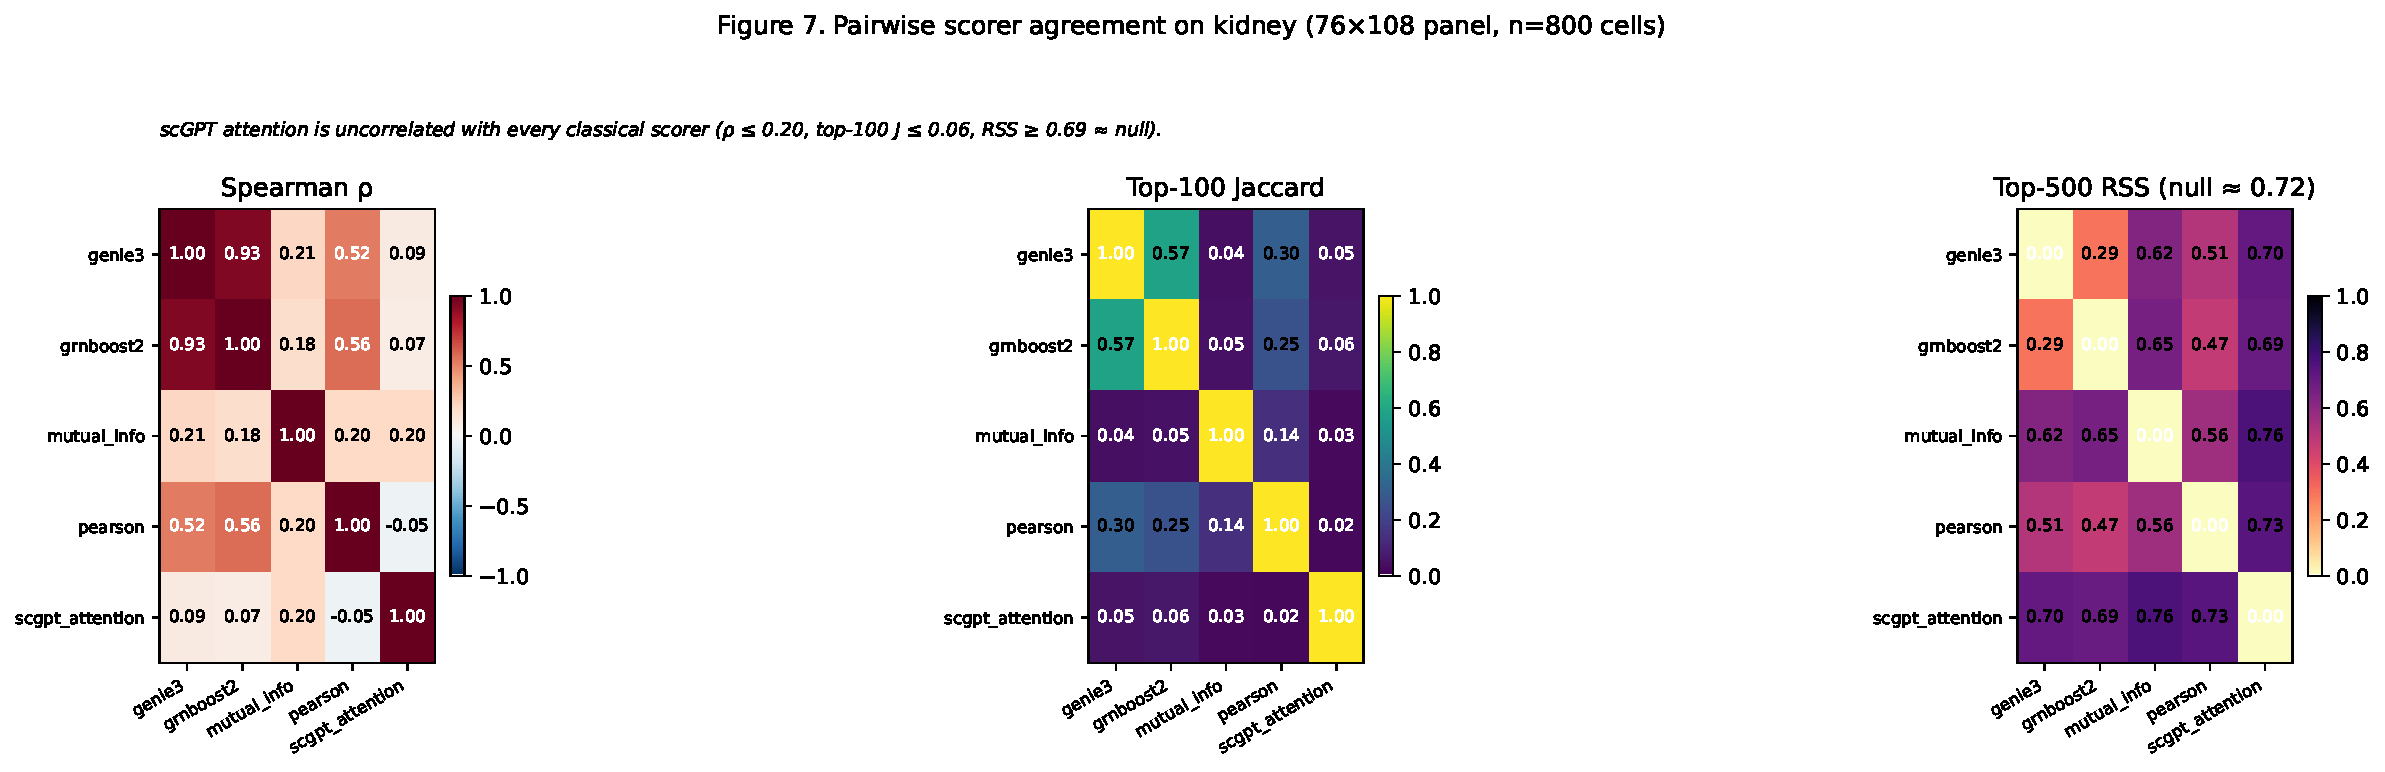
\includegraphics[width=\textwidth]{figures/fig7_scorer_divergence.pdf}
\caption{\textbf{Pairwise scorer agreement on kidney}
(hematopoiesis $76 \times 108$ panel, $n = 800$ cells).
Left: Spearman $\rho$. Centre: top-100 Jaccard. Right: top-500 RSS
composite (null mean $\approx 0.72$, shown in darker red). scGPT
attention is uncorrelated with every classical scorer (last row/column);
GRNBoost2 and GENIE3 are nearly identical.}
\label{fig:scorer_divergence}
\end{figure*}

\begin{table*}[ht]
\centering
\caption{Pairwise scorer-agreement matrix on kidney
(76 TFs $\times$ 99 targets panel, $n = 800$ cells). All top-500 RSS
values should be compared against the rank-permutation null mean of
$\approx 0.72$: values far below null indicate concordant rankings,
values near null indicate ranking independence.}
\label{tab:scorer_divergence}
\small
\begin{tabular}{llrrrr}
\toprule
\textbf{Scorer A} & \textbf{Scorer B} & \textbf{Spearman} & \textbf{Top-100 J} & \textbf{Top-500 J} & \textbf{Top-500 RSS} \\
\midrule
Pearson & Mutual info        & 0.20  & 0.14 & 0.21 & 0.56 \\
Pearson & GRNBoost2          & 0.56  & 0.25 & 0.32 & 0.47 \\
Pearson & GENIE3             & 0.52  & 0.30 & 0.26 & 0.51 \\
Pearson & scGPT attention    & $-$0.05 & 0.02 & 0.04 & \textbf{0.73} \\
Mutual info & GRNBoost2      & 0.18  & 0.05 & 0.14 & 0.65 \\
Mutual info & GENIE3         & 0.21  & 0.04 & 0.16 & 0.62 \\
Mutual info & scGPT attention & 0.20 & 0.03 & 0.06 & \textbf{0.76} \\
GRNBoost2 & GENIE3           & 0.93  & 0.58 & 0.54 & 0.29 \\
GRNBoost2 & scGPT attention  & 0.07  & 0.06 & 0.06 & \textbf{0.69} \\
GENIE3 & scGPT attention     & 0.09  & 0.05 & 0.05 & \textbf{0.70} \\
\bottomrule
\end{tabular}
\end{table*}

\subsection{Cross-axis analysis}

\DIFadd{The five axes are not independent
(}\DIFaddend Table~\ref{tab:fragility}\DIFdelbegin \DIFdel{summarizes the per-axis robustness profile
across all datasets, and }\DIFdelend \DIFaddbegin \DIFadd{, }\DIFaddend Figure~\ref{fig:crossaxis}\DIFdelbegin \DIFdel{visualizes the pass/marginal/fail
status for each axis--dataset combination. Several cross-axis interactions are worth
highlighting. }%DIFDELCMD < 

%DIFDELCMD < %%%
\DIFdel{First, the cell-count axis and the rare-type axis }\DIFdelend \DIFaddbegin \DIFadd{). Three
interactions matter for practice. First, Axis~1 and Axis~3 }\DIFaddend are
mechanistically linked \DIFdelbegin \DIFdel{: because
unconstrained inference requires $>$}\DIFdelend \DIFaddbegin \DIFadd{under scGPT attention: rare types ($<\!500$
cells) operate below the scGPT MVCC of $\sim$}\DIFaddend 3{,}000\DIFdelbegin \DIFdel{cells for stability (Axis~1), and most rare
cell types contain far fewer than 500 cells, rare types are inherently operating in the
unstable regime, which provides a partial mechanistic explanation for }\DIFdelend \DIFaddbegin \DIFadd{, partly
explaining }\DIFaddend their 0\% reliability-gate passage\DIFdelbegin \DIFdel{in Axis~3.
}%DIFDELCMD < 

%DIFDELCMD < %%%
\DIFdelend \DIFaddbegin \DIFadd{; under Pearson and tree
scorers (MVCC 200--500) the link is weaker, so the rare-vs-abundant
gap is also driven by sparsity and lower null-separation in small
subsamples. }\DIFaddend Second, the \DIFdelbegin \DIFdel{choice of clustering resolution (}\DIFdelend \DIFaddbegin \DIFadd{dual-null coarse recommendation from }\DIFaddend Axis~2
\DIFdelbegin \DIFdel{) affects donor generalization
(}\DIFdelend \DIFaddbegin \DIFadd{indirectly aids }\DIFaddend Axis~4\DIFdelbegin \DIFdel{) in a subtle way: }\DIFdelend \DIFaddbegin \DIFadd{, since }\DIFaddend coarse clustering pools cell-type
variation that would otherwise \DIFdelbegin \DIFdel{need to be controlled through }\DIFdelend \DIFaddbegin \DIFadd{require }\DIFaddend per-donor composition matching.
\DIFdelbegin \DIFdel{This suggests
that the universal coarse-clustering recommendation from dual-null calibration may
confer indirect benefits for cross-donor robustness as well.
}%DIFDELCMD < 

%DIFDELCMD < %%%
\DIFdel{Third, integration (}\DIFdelend \DIFaddbegin \DIFadd{Third, }\DIFaddend Axis~5 \DIFdelbegin \DIFdel{) }\DIFdelend operates upstream of \DIFdelbegin \DIFdel{all other axes }\DIFdelend \DIFaddbegin \DIFadd{every other axis }\DIFaddend by altering the
correlation structure on which \DIFdelbegin \DIFdel{edge }\DIFdelend scores are computed\DIFdelbegin \DIFdel{. Harmony's rank perturbation
therefore has the potential to cascade into cell-count stability, resolution sensitivity,
and rare-type null separation, making integration
}\DIFdelend \DIFaddbegin \DIFadd{, so integration
choice is }\DIFaddend a latent confounder for \DIFdelbegin \DIFdel{all other
axes. }%DIFDELCMD < 

%DIFDELCMD < %%%
\DIFdel{The most striking finding is that no }\DIFdelend \DIFaddbegin \DIFadd{cell-count, resolution, and rare-type
calibrations. No }\DIFaddend dataset passes all five axes under their \DIFdelbegin \DIFdel{respective
calibrated
criteria . Every tissue fails at least two axes, and there is }\DIFdelend \DIFaddbegin \DIFadd{calibrated
criteria in any single scorer family, }\DIFaddend no single corrective measure
\DIFdelbegin \DIFdel{(more cells, coarser clustering, more donors, or integration) that
}\DIFdelend resolves all fragilities\DIFdelbegin \DIFdel{simultaneously. This reinforces the paper's central message}\DIFdelend \DIFaddbegin \DIFadd{, and within-scorer fragility profiles do not
transfer across scorer families}\DIFaddend : robustness must be demonstrated, not
assumed, along each axis \DIFdelbegin \DIFdel{relevant to a given study}\DIFdelend \DIFaddbegin \emph{\DIFadd{and}} \DIFadd{each scorer choice}\DIFaddend .

\DIFdelbegin %DIFDELCMD < \begin{figure}[ht]
%DIFDELCMD < \centering
%DIFDELCMD < 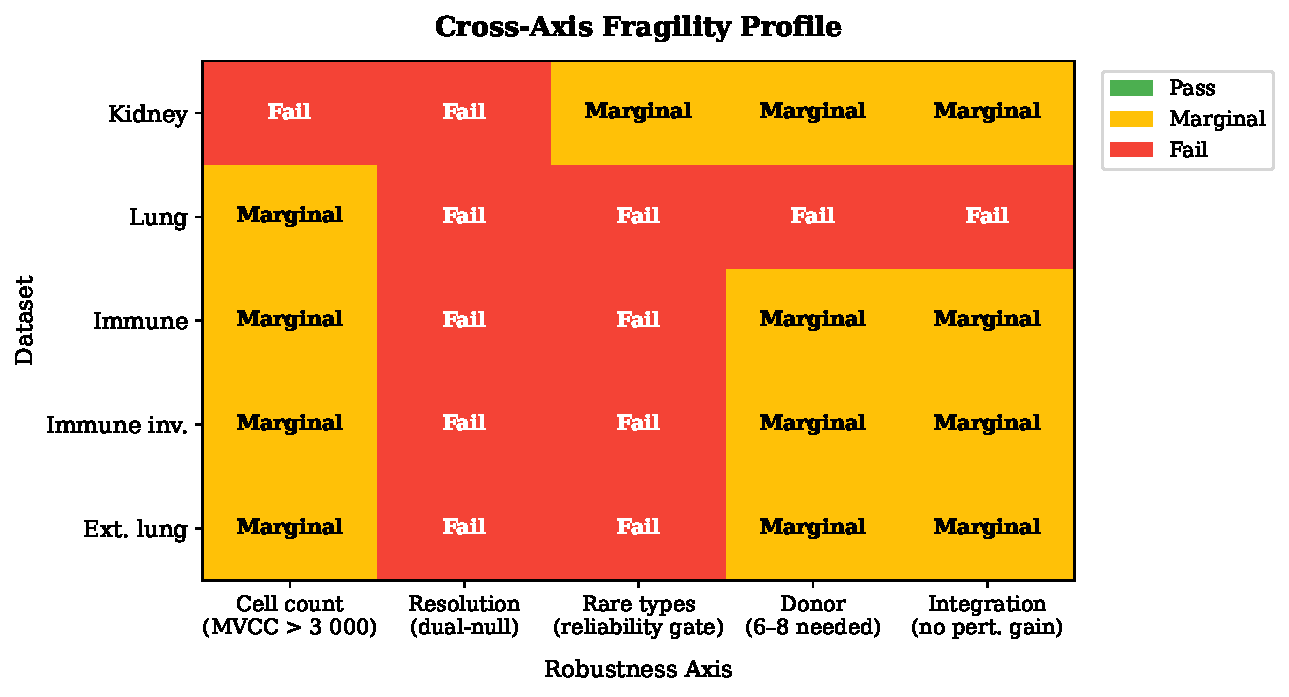
\includegraphics[width=0.85\textwidth]{figures/fig6_cross_axis.pdf}
%DIFDELCMD < \caption{\textbf{Cross-axis fragility summary.}
%DIFDELCMD < Heatmap showing pass (green), marginal (yellow), and fail (red) status for each
%DIFDELCMD < axis--dataset combination under calibrated criteria.}
%DIFDELCMD < \label{fig:crossaxis}
%DIFDELCMD < \end{figure}
%DIFDELCMD < %%%
\DIFdelend \DIFaddbegin \begin{figure*}[ht]
\centering
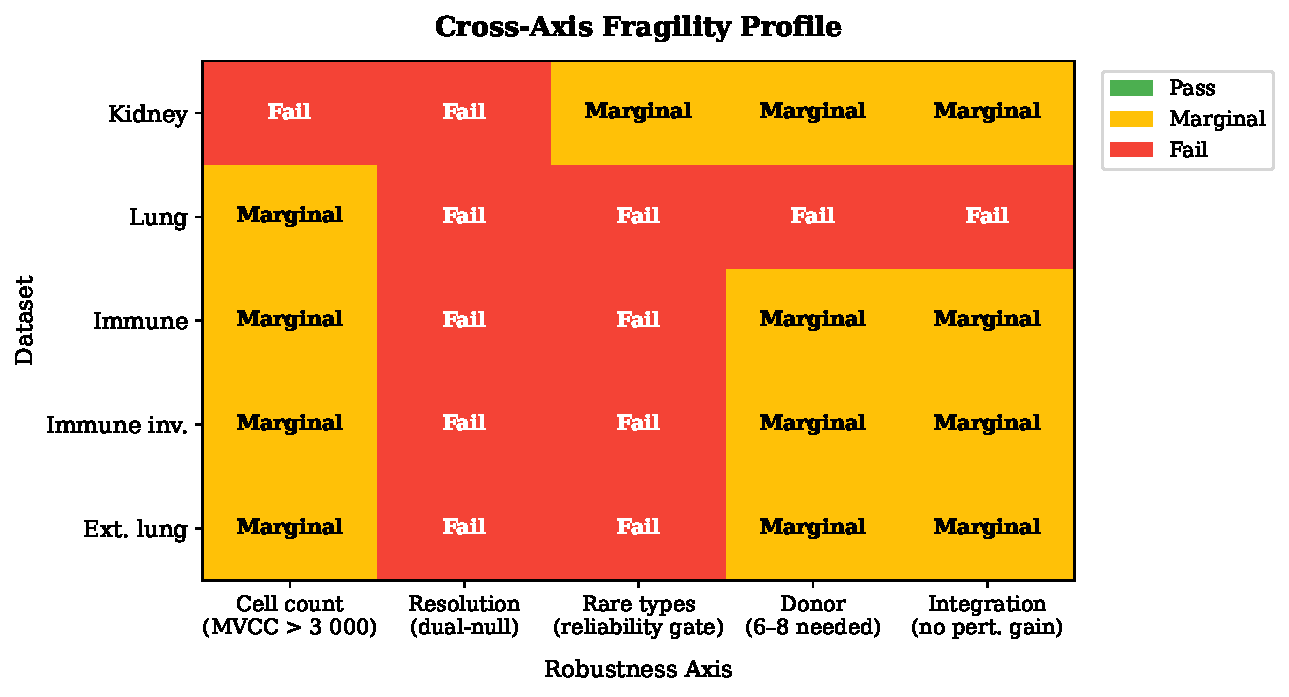
\includegraphics[width=0.85\textwidth]{figures/fig6_cross_axis.pdf}
\caption{\textbf{Cross-axis fragility summary.}
Heatmap showing pass (green), marginal (yellow), and fail (red) status for each
axis--dataset combination under calibrated criteria.}
\label{fig:crossaxis}
\end{figure*}
\DIFaddend 

\DIFdelbegin %DIFDELCMD < \begin{table}[ht]
%DIFDELCMD < \centering
%DIFDELCMD < \caption{Per-axis robustness summary with key metric, calibrated threshold, and practical recommendation.}
%DIFDELCMD < \label{tab:fragility}
%DIFDELCMD < \small
%DIFDELCMD < \begin{tabularx}{\textwidth}{lXlX}
%DIFDELCMD < \toprule
%DIFDELCMD < \textbf{Axis} & \textbf{Key Metric} & \textbf{Threshold} & \textbf{Recommendation} \\
%DIFDELCMD < \midrule
%DIFDELCMD < Cell count & MVCC (top-1k Jaccard $>$ 0.5) & $>$3{,}000 cells &
%DIFDELCMD <   Use $\geq$3{,}000 cells or apply prior constraints \\
%DIFDELCMD < \addlinespace
%DIFDELCMD < Resolution & Dual-null pass rate & Both nulls must pass &
%DIFDELCMD <   Default to coarse; report within-class heterogeneity \\
%DIFDELCMD < \addlinespace
%DIFDELCMD < Rare types & Reliability gate (5 criteria) & All must pass &
%DIFDELCMD <   Treat rare-cell edges as hypothesis-generating only \\
%DIFDELCMD < \addlinespace
%DIFDELCMD < Donor & Fixed-holdout Spearman & 90\% of best & Collect $\geq$6 donors (8 conservative) \\
%DIFDELCMD < \addlinespace
%DIFDELCMD < Integration & Perturbation swap $\Delta$ & FDR $<$ 0.05 &
%DIFDELCMD <   Report multi-reference validation; avoid universal claims \\
%DIFDELCMD < \bottomrule
%DIFDELCMD < \end{tabularx}
%DIFDELCMD < \end{table}
%DIFDELCMD < %%%
\DIFdelend \DIFaddbegin \begin{table*}[ht]
\centering
\caption{Per-axis robustness summary: calibrated criterion and practical recommendation.}
\label{tab:fragility}
\small
\begin{tabularx}{\textwidth}{@{}l X X@{}}
\toprule
\textbf{Axis} & \textbf{Calibrated criterion} & \textbf{Recommendation} \\
\midrule
Cell count   & MVCC (top-1k Jaccard $>0.5$); scorer-dependent: 200 cells (Pearson / tree, 4 of 6 cohorts), 500 cells (Pearson, primary immune and Delorey COVID lung), $>$3{,}000 cells (scGPT attention, anchor-invariant) & Use the MVCC for your chosen scorer family; apply DoRothEA-constrained policies to rescue small-sample scGPT runs \\
\addlinespace
Resolution   & Dual-null pass: both global cell-label shuffle and within-coarse constrained shuffle must clear at empirical $p \leq 0.05$ & Default to coarse; report within-class RSS heterogeneity \\
\addlinespace
Rare types   & Reliability gate: stability $\geq 0.75$, top-$k$ Jaccard $\geq 0.35$, null AUC $\geq 0.65$, positive tail gap, cell count $\geq 80$ & Treat rare-cell-type edges as hypothesis-generating only \\
\addlinespace
Donor        & Fixed-holdout Spearman $\geq$ 90\% of best (300 cells/donor) & Collect $\geq 6$ donors (8 for conservative generalisation) \\
\addlinespace
Integration  & Paired-swap $\Delta$ precision against curated reference, BH-FDR $<0.05$ & Report multi-reference validation; avoid universal claims of biological gain \\
\bottomrule
\end{tabularx}
\end{table*}
\DIFaddend 

% ============================================================
% 4. DISCUSSION
% ============================================================
\section{Discussion}

This audit demonstrates that GRN edge rankings from single-cell data are fragile
along multiple axes simultaneously, and that apparent robustness along one axis
(e.g., coarse rank stability for rare types) can mask failure along another
(e.g., null separation). The adversarial-review methodology that we applied to
each axis is itself a contribution: by requiring corrective experiments before
claims are updated, it systematically closes the gap between initial findings and
defensible conclusions.

\paragraph{Practical implications.}
Table~\ref{tab:guidelines} provides concrete guidance\DIFdelbegin \DIFdel{for practitioners.
The central message is that }\DIFdelend \DIFaddbegin \DIFadd{: }\DIFaddend no single
parameter choice can guarantee robust GRN inference; \DIFdelbegin \DIFdel{instead, }\DIFdelend robustness must
be demonstrated along each relevant axis for the specific tissue,
cell count, and analytical choices at hand.

\DIFdelbegin %DIFDELCMD < \begin{table}[ht]
%DIFDELCMD < \centering
%DIFDELCMD < \caption{Practical guidelines for robust GRN inference from single-cell data.}
%DIFDELCMD < \label{tab:guidelines}
%DIFDELCMD < \small
%DIFDELCMD < \begin{tabularx}{\textwidth}{lX}
%DIFDELCMD < \toprule
%DIFDELCMD < \textbf{Decision Point} & \textbf{Guideline} \\
%DIFDELCMD < \midrule
%DIFDELCMD < \textit{Sample size} &
%DIFDELCMD <   Target $\geq$3{,}000 cells for unconstrained inference, or use informative prior
%DIFDELCMD <   constraints (DoRothEA/TRRUST) which stabilize rankings at 200+ cells. \\
%DIFDELCMD < \addlinespace
%DIFDELCMD < \textit{Clustering} &
%DIFDELCMD <   Default to coarse clustering unless dual-null calibration (global + within-coarse
%DIFDELCMD <   constrained shuffle) confirms that fine resolution adds separable signal. Report
%DIFDELCMD <   within-class RSS for compartment-level uncertainty. \\
%DIFDELCMD < \addlinespace
%DIFDELCMD < \textit{Rare cell types} &
%DIFDELCMD <   Report null-separation AUC alongside stability for every cell type. Flag rare types
%DIFDELCMD <   ($< 250$ cells) as hypothesis-generating. Provide minimum-reliable-size estimates
%DIFDELCMD <   with uncertainty status. \\
%DIFDELCMD < \addlinespace
%DIFDELCMD < \textit{Donor coverage} &
%DIFDELCMD <   Collect $\geq$6 donors (8 for conservative generalization). Use fixed-holdout
%DIFDELCMD <   evaluation, not complementary splits. Report composition-controlled transfer alongside
%DIFDELCMD <   raw transfer. \\
%DIFDELCMD < \addlinespace
%DIFDELCMD < \textit{Integration} &
%DIFDELCMD <   Report at least paired swap significance for reference gains, plus one
%DIFDELCMD <   perturbation-backed metric when available. Include hyperparameter sensitivity
%DIFDELCMD <   ($n_{\text{pcs}}$). Avoid universal claims of biological improvement. \\
%DIFDELCMD < \addlinespace
%DIFDELCMD < \textit{Cross-axis audit} &
%DIFDELCMD <   Report a fragility profile (Table~\ref{tab:fragility}) covering all axes relevant to
%DIFDELCMD <   the study design. Acknowledge which axes were not testable and why. \\
%DIFDELCMD < \bottomrule
%DIFDELCMD < \end{tabularx}
%DIFDELCMD < \end{table}
%DIFDELCMD < %%%
\DIFdelend \DIFaddbegin \begin{table*}[ht]
\centering
\caption{Practical guidelines for robust GRN inference from single-cell data.}
\label{tab:guidelines}
\small
\begin{tabularx}{\textwidth}{lX}
\toprule
\textbf{Decision Point} & \textbf{Guideline} \\
\midrule
\textit{Sample size} &
  Target $\geq 3{,}000$ cells under scGPT attention or use informative
  prior constraints (DoRothEA / TRRUST) which stabilise scGPT rankings
  at 200+ cells. Under Pearson, mutual-information, and tree-based
  scorers, 200--500 cells are often sufficient on the cohorts tested;
  verify per-scorer MVCC before committing. \\
\addlinespace
\textit{Clustering} &
  Default to coarse clustering unless a dual-null calibration (global +
  within-coarse constrained shuffle) confirms that fine resolution
  adds separable signal; in our six cohorts, no coarse-vs-fine
  configuration cleared both nulls, so every recommendation collapses
  to coarse or hybrid. Report within-class RSS for compartment-level
  uncertainty. \\
\addlinespace
\textit{Rare cell types} &
  Report null-separation AUC alongside rank stability for every cell
  type; a high Spearman stability can coexist with null-level AUC
  (Delorey COVID cohort, §3.3). Flag rare types ($< 250$ cells) as
  hypothesis-generating. Provide minimum-reliable-size estimates with
  uncertainty status. \\
\addlinespace
\textit{Donor coverage} &
  Collect $\geq 6$ donors under strict cells-per-donor balancing
  (300 cells/donor, 8 donors for conservative generalisation); under
  looser balancing (200 cells/donor), the requirement drops to 2--4
  donors. State the cells-per-donor policy explicitly. Use
  fixed-holdout evaluation, not complementary splits, and report
  composition-controlled transfer alongside raw transfer. \\
\addlinespace
\textit{Integration} &
  Run at least two integration methods on the same cells, not only the
  tool that happens to be most popular in the pipeline: we observe
  Spearman ranging from 0.06 (Scanorama on kidney) to 0.87 (Harmony
  on immune) on identical inputs. Report at least paired swap
  significance for reference gains, plus one perturbation-backed
  metric when available, and include a hyperparameter-sensitivity
  sweep. Avoid universal claims of biological improvement. \\
\addlinespace
\textit{Scorer choice} &
  Auditing one scorer does not license conclusions about another: in
  our kidney experiment, scGPT-attention rankings overlap with Pearson
  rankings in fewer than 5\% of top-100 edges. Re-audit every axis
  under the scorer used to generate the published rankings. \\
\addlinespace
\textit{Cross-axis audit} &
  Report a fragility profile (Table~\ref{tab:fragility}) covering all
  axes relevant to the study design. Acknowledge which axes were not
  testable and why. \\
\bottomrule
\end{tabularx}
\end{table*}
\DIFaddend 

\paragraph{Comparison to existing benchmarks.}
Published GRN benchmarks~\DIFdelbegin \DIFdel{\mbox{%DIFAUXCMD
\citep{Pratapa2020, Chen2023} }\hskip0pt%DIFAUXCMD
}\DIFdelend \DIFaddbegin \DIFadd{\mbox{%DIFAUXCMD
\citep{Pratapa2020, Chen2018} }\hskip0pt%DIFAUXCMD
}\DIFaddend have focused primarily on
accuracy relative to gold-standard references, treating preprocessing as fixed.
Our audit complements these by asking whether rankings are \emph{stable} across
realistic analytical perturbations, a necessary condition for practical utility.
The two perspectives are not redundant: a method can be accurate under one
configuration and fragile under perturbation, or robustly mediocre across all
configurations.

\paragraph{Limitations.}
\DIFdelbegin \DIFdel{Several limitations apply across the audit. First, all edge scoring is
correlation-based and does not }\DIFdelend \DIFaddbegin \DIFadd{None of the five scorers }\DIFaddend directly estimate causal regulatory effects;
\DIFdelbegin \DIFdel{although }\DIFdelend correlation on normalized counts avoids zero-inflation
artifacts~\citep{Svensson2020} \DIFdelbegin \DIFdel{, it }\DIFdelend \DIFaddbegin \DIFadd{but }\DIFaddend remains susceptible to confounding
by shared upstream regulators~\citep{Kharchenko2014}\DIFdelbegin \DIFdel{.
Second, the audit covers }\DIFdelend \DIFaddbegin \DIFadd{, tree-ensemble
scorers introduce their own biases, and scGPT attention reflects
pretraining patterns on the CellxGene Census rather than causal edges.
The audit covers four }\DIFaddend Tabula Sapiens tissues \DIFdelbegin \DIFdel{and one external lung cohort;
generalization to }\DIFdelend \DIFaddbegin \DIFadd{plus one external-lab
SmartSeq2 lung cohort and one COVID-19 lung disease cohort;
generalisation to other }\DIFaddend disease tissues, developmental atlases, \DIFdelbegin \DIFdel{or }\DIFdelend \DIFaddbegin \DIFadd{and
}\DIFaddend cross-species comparisons remains untested. \DIFdelbegin \DIFdel{Third, adversarial null designs (particularly
constrained shuffles) may be overly strict for certain scoring families ,
potentially leading to conservative recommendations that reject genuine fine-scale
signal. Fourth, perturbation-backed validation data remain sparse, limiting
statistical powerfor perturbation swap tests. Fifth, we evaluated only
Harmony among integration methods ; broader comparisons including scVIand
Scanorama~\mbox{%DIFAUXCMD
\citep{Gayoso2022, Hie2019}}\hskip0pt%DIFAUXCMD
,
guided by recent }\DIFdelend \DIFaddbegin \DIFadd{The within-coarse null is
demanding and other scoring families might clear it; the
single-cell-DE literature documents how easily under-calibrated nulls
inflate apparent
discoveries~\mbox{%DIFAUXCMD
\citep{Squair2021}}\hskip0pt%DIFAUXCMD
, supporting the within-coarse stringency
we adopt. Perturbation-backed validation remains data-sparse, limiting
swap-test power. Three integration methods are compared side-by-side
(Harmony~\mbox{%DIFAUXCMD
\citep{Korsunsky2019}}\hskip0pt%DIFAUXCMD
, scVI~\mbox{%DIFAUXCMD
\citep{Gayoso2022}}\hskip0pt%DIFAUXCMD
,
Scanorama~\mbox{%DIFAUXCMD
\citep{Hie2019}}\hskip0pt%DIFAUXCMD
); broader }\DIFaddend integration
benchmarks~\citep{Luecken2022, Tran2020} \DIFdelbegin \DIFdel{, are warranted}\DIFdelend \DIFaddbegin \DIFadd{and recent multimodal
integration frameworks~\mbox{%DIFAUXCMD
\citep{Hao2024} }\hskip0pt%DIFAUXCMD
suggest extending the
cross-method comparison further is a natural next step}\DIFaddend .

% ============================================================
% 5. CONCLUSION
% ============================================================
\section{Conclusion}

\DIFdelbegin \DIFdel{We present the first systematic }\DIFdelend \DIFaddbegin \DIFadd{This systematic multi-scorer, }\DIFaddend multi-axis robustness audit of
\DIFdelbegin \DIFdel{GRN inference from
single-cell transcriptomics, spanning }\DIFdelend \DIFaddbegin \DIFadd{single-cell GRN inference --- five scorers, six cohorts, five axes
(}\DIFaddend cell count, clustering resolution, rare-cell reliability, donor
\DIFdelbegin \DIFdel{generalization, and integration-method sensitivity. The audit
reveals that fragility is }\DIFdelend \DIFaddbegin \DIFadd{generalisation, integration sensitivity) --- finds fragility to be
}\DIFaddend pervasive, axis-specific, \DIFdelbegin \DIFdel{and interactive: no dataset
passed }\DIFdelend \DIFaddbegin \DIFadd{interactive, and scorer-specific. No dataset
passes }\DIFaddend all five axes under calibrated criteria \DIFdelbegin \DIFdel{, }\DIFdelend \DIFaddbegin \DIFadd{in any scorer family;
the within-coarse resolution null fails universally under dual- }\DIFaddend and
\DIFdelbegin \DIFdel{corrective measures along one
axis do not automatically resolve others. We provide a practical guidelines table
and an open-source framework, consisting of modular Python scripts for each axis
(subsampling sweeps, resolution calibration with dual nulls, rare-type reliability
gates, donor-holdout curves, and integration swap tests), that enables }\DIFdelend \DIFaddbegin \DIFadd{triple-null calibrations; the rare-vs-abundant reliability gap holds
across 5}{\DIFadd{,}}\DIFadd{880 threshold combinations; and scGPT attention rankings
are statistically uncorrelated with classical-scorer rankings on the
same cells. The accompanying }\texttt{\DIFadd{fragility}} \DIFadd{package reproduces
every CSV and figure from raw h5ad via a single }\texttt{\DIFadd{make audit}}
\DIFadd{command and is extensible to new scorers and datasets through a single
interface; we encourage }\DIFaddend practitioners to conduct analogous audits
\DIFdelbegin \DIFdel{for their own datasets and inference pipelines }\DIFdelend before publishing GRN claims.

% ============================================================
% AUTHOR CONTRIBUTIONS
% ============================================================
\section*{Author Contributions}

\DIFdelbegin \DIFdel{I.K.\ conceived the study, designed the five-axis robustness audit framework, implemented all computational pipelines,
performed all statistical analyses, generated all figures and tables, and wrote the manuscript}\DIFdelend \DIFaddbegin \textbf{\DIFadd{Ihor Kendiukhov:}} \DIFadd{Conceptualization, Methodology, Software,
Formal analysis, Investigation, Data curation, Writing -- original
draft, Writing -- review \& editing, Visualization, Project administration}\DIFaddend .

% ============================================================
% ACKNOWLEDGEMENTS
% ============================================================
\section*{Acknowledgements}

The author thanks the Tabula Sapiens Consortium \DIFaddbegin \DIFadd{and the authors of
the Travaglini et al.\ 2020 lung atlas and the Delorey et al.\ 2021
COVID-19 lung atlas }\DIFaddend for making their single-cell \DIFdelbegin \DIFdel{atlas publicly
available}\DIFdelend \DIFaddbegin \DIFadd{data publicly
available, and the authors of scGPT and the DoRothEA / TRRUST
databases for releasing their tools and references under open
licences}\DIFaddend .

% ============================================================
% FUNDING
% ============================================================
\section*{Funding}

This work was not supported by any specific grant from funding agencies in the
public, commercial, or not-for-profit sectors. No external funding was received.

% ============================================================
% CONFLICT OF INTEREST
% ============================================================
\section*{Conflict of Interest}

None declared.

% ============================================================
% DATA AND CODE AVAILABILITY
% ============================================================
\section*{Data and Code Availability}

\DIFdelbegin \DIFdel{All }\DIFdelend \DIFaddbegin \DIFadd{The unified }\texttt{\DIFadd{fragility}} \DIFadd{package (}\DIFaddend source code, analysis
pipelines, \DIFdelbegin \DIFdel{result tables, and figure-generation scriptsare }\DIFdelend \DIFaddbegin \DIFadd{null library, metric definitions, panel registry, scorer
implementations, and figure-regeneration scripts) is }\DIFaddend publicly available
at \url{https://github.com/Biodyn-AI/grn-robustness-audit} \DIFdelbegin \DIFdel{.
}\DIFdelend \DIFaddbegin \DIFadd{and a
versioned archive of the code accompanying this submission is deposited
on Zenodo at }\url{https://doi.org/10.5281/zenodo.20009065}\DIFadd{. A single
}\texttt{\DIFadd{make audit}} \DIFadd{command reproduces every CSV and figure in this
paper from raw h5ad input.
}

\DIFaddend Raw single-cell data are from the \DIFaddbegin \DIFadd{following public sources: }\DIFaddend Tabula
Sapiens Consortium \DIFdelbegin \DIFdel{and are available at
}\DIFdelend \DIFaddbegin \DIFadd{(}\DIFaddend \url{https://tabula-sapiens-portal.ds.czbiohub.org/}\DIFaddbegin \DIFadd{);
Travaglini et al.\ 2020 SmartSeq2 lung atlas (CellxGene); and
Delorey et al.\ 2021 COVID-19 lung atlas (CellxGene dataset
}\texttt{\DIFadd{75c059c8-8fb7-4e6e-a618-a3e01ac42060}}\DIFadd{).
The scGPT }\emph{\DIFadd{whole-human}} \DIFadd{checkpoint is from
\mbox{%DIFAUXCMD
\citet{Cui2024}}\hskip0pt%DIFAUXCMD
; the DoRothEA and TRRUST panels are from
\mbox{%DIFAUXCMD
\citet{GarciaAlonso2019} }\hskip0pt%DIFAUXCMD
and \mbox{%DIFAUXCMD
\citet{Han2018} }\hskip0pt%DIFAUXCMD
respectively}\DIFaddend .

% ============================================================
% SUPPLEMENTARY INFORMATION
% ============================================================
\section*{Supplementary Information}

Supplementary \DIFdelbegin \DIFdel{tables with per-dataset, per-axis detailed metrics and the full
hyperparameter-grid results are available }\DIFdelend \DIFaddbegin \DIFadd{Methods S1 contains the panel registry (gene lists for
every named TF--target panel used in the paper) and extended
preprocessing documentation. Supplementary Methods S2 describes the
adversarial AI-assisted review protocol, including base model, prompt
rubric, round-by-round logs, and the full-census 27-issue classification
under the pre-registered rubric. Supplementary Figures S1--S7 cover,
respectively: the full MVCC anchor ablation; the RSS weight-simplex
sweep; the rank-permutation empirical null distribution; the
5}{\DIFadd{,}}\DIFadd{880-point reliability-gate threshold-sensitivity heatmap; the
top-$k$ scan over $k \in \{100, 500, 1{,}000, 5{,}000,$ 1\%, 5\%,
10\%$\}$; the normalization ablation (depth / size-factor / Pearson
residuals); and the triple-null calibration. Supplementary Table~S3
reports Axis-3 per-cell-type reliability metrics under the shared
primary panel for all Tabula Sapiens cohorts. All supplementary
material is available at }\textit{\DIFadd{Bioinformatics}} \DIFadd{online and }\DIFaddend in the
GitHub repository.

% ============================================================
% ABBREVIATIONS
% ============================================================
\section*{Abbreviations}

\noindent
AUC: Area Under the Curve;
BH: Benjamini--Hochberg;
FDR: False Discovery Rate;
GRN: Gene Regulatory Network;
MVCC: Minimum Valid Cell Count;
PCA: Principal Component Analysis;
RSS: Resolution Sensitivity Score;
scRNA-seq: Single-Cell RNA Sequencing;
TF: Transcription Factor.

% ============================================================
% REFERENCES
% ============================================================
\begin{thebibliography}{99}

\bibitem[Aibar et~al., 2017]{Aibar2017}
Aibar, S., Gonz{\'a}lez-Blas, C.~B., Moerman, T., et~al. (2017).
\newblock SCENIC: single-cell regulatory network inference and clustering.
\newblock \textit{Nature Methods}, 14(11):1083--1086.

\DIFdelbegin \bibitem[Chen and Mar, 2018]{Chen2023}
\DIFdelend \DIFaddbegin \bibitem[Benjamini and Hochberg, 1995]{BenjaminiHochberg1995}
\DIFadd{Benjamini, Y. and Hochberg, Y. (1995).
}\newblock \DIFadd{Controlling the false discovery rate: a practical and powerful
  approach to multiple testing.
}\newblock \textit{\DIFadd{Journal of the Royal Statistical Society: Series B
  (Methodological)}}\DIFadd{, 57(1):289--300.
}

\bibitem[Chen and Mar, 2018]{Chen2018}
\DIFaddend Chen, S. and Mar, J.~C. (2018).
\newblock Evaluating methods of inferring gene regulatory networks highlights
  their lack of performance for single cell gene expression data.
\newblock \textit{BMC Bioinformatics}, 19(1):232.

\bibitem[Cui et~al., 2024]{Cui2024}
Cui, H., Wang, C., Maan, H., et~al. (2024).
\newblock scGPT: toward building a foundation model for single-cell multi-omics
  using generative AI.
\newblock \textit{Nature Methods}, 21(8):1470--1480.

\DIFaddbegin \bibitem[Delorey et~al., 2021]{Delorey2021}
\DIFadd{Delorey, T.~M., Ziegler, C.~G.~K., Heimberg, G., et~al. (2021).
}\newblock \DIFadd{COVID-19 tissue atlases reveal SARS-CoV-2 pathology and cellular
  targets.
}\newblock \textit{\DIFadd{Nature}}\DIFadd{, 595(7865):107--113.
}

\DIFaddend \bibitem[Dixit et~al., 2016]{Dixit2016}
Dixit, A., Parnas, O., Li, B., et~al. (2016).
\newblock Perturb-Seq: \DIFdelbegin \DIFdel{Dissecting }\DIFdelend \DIFaddbegin \DIFadd{dissecting }\DIFaddend molecular circuits with scalable single-cell
  RNA profiling of pooled genetic screens.
\newblock \textit{Cell}, 167(7):1853--1866.\DIFaddbegin \DIFadd{e17.
}\DIFaddend 

\bibitem[Garcia-Alonso et~al., 2019]{GarciaAlonso2019}
Garcia-Alonso, L., Holland, C.~H., Ibrahim, M.~M., Turei, D., and
  Saez-Rodriguez, J. (2019).
\newblock Benchmark and integration of resources for the estimation of human
  transcription factor activities.
\newblock \textit{Genome Research}, 29(8):1363--1375.

\bibitem[Gayoso et~al., 2022]{Gayoso2022}
Gayoso, A., Lopez, R., Xing, G., et~al. (2022).
\newblock A Python library for probabilistic analysis of single-cell omics data.
\newblock \textit{Nature Biotechnology}, 40(2):163--166.

\DIFaddbegin \bibitem[Haghverdi et~al., 2018]{Haghverdi2018}
\DIFadd{Haghverdi, L., Lun, A.~T.~L., Morgan, M.~D., and Marioni, J.~C. (2018).
}\newblock \DIFadd{Batch effects in single-cell RNA-sequencing data are corrected by
  matching mutual nearest neighbors.
}\newblock \textit{\DIFadd{Nature Biotechnology}}\DIFadd{, 36(5):421--427.
}

\DIFaddend \bibitem[Han et~al., 2018]{Han2018}
Han, H., Cho, J.-W., Lee, S., et~al. (2018).
\newblock TRRUST v2: an expanded reference database of human and mouse
  transcriptional regulatory interactions.
\newblock \textit{Nucleic Acids Research}, 46(D1):\DIFdelbegin \DIFdel{D199--D202}\DIFdelend \DIFaddbegin \DIFadd{D380--D386}\DIFaddend .

\DIFaddbegin \bibitem[Hao et~al., 2024]{Hao2024}
\DIFadd{Hao, Y., Stuart, T., Kowalski, M.~H., et~al. (2024).
}\newblock \DIFadd{Dictionary learning for integrative, multimodal and scalable
  single-cell analysis.
}\newblock \textit{\DIFadd{Nature Biotechnology}}\DIFadd{, 42(2):293--304.
}

\bibitem[Heumos et~al., 2023]{Heumos2023}
\DIFadd{Heumos, L., Schaar, A.~C., Lance, C., et~al. (2023).
}\newblock \DIFadd{Best practices for single-cell analysis across modalities.
}\newblock \textit{\DIFadd{Nature Reviews Genetics}}\DIFadd{, 24(8):550--572.
}

\DIFaddend \bibitem[Hie et~al., 2019]{Hie2019}
Hie, B., Bryson, B., and Berger, B. (2019).
\newblock Efficient integration of heterogeneous single-cell transcriptomes
  using Scanorama.
\newblock \textit{Nature Biotechnology}, 37(6):685--691.

\DIFaddbegin \bibitem[Huynh-Thu et~al., 2010]{Huynh-Thu2010}
\DIFadd{Huynh-Thu, V.~A., Irrthum, A., Wehenkel, L., and Geurts, P. (2010).
}\newblock \DIFadd{Inferring regulatory networks from expression data using tree-based
  methods.
}\newblock \textit{\DIFadd{PLoS ONE}}\DIFadd{, 5(9):e12776.
}

\DIFaddend \bibitem[Kharchenko et~al., 2014]{Kharchenko2014}
Kharchenko, P.~V., Silberstein, L., and Scadden, D.~T. (2014).
\newblock Bayesian approach to single-cell differential expression analysis.
\newblock \textit{Nature Methods}, 11(7):740--742.

\bibitem[Korsunsky et~al., 2019]{Korsunsky2019}
Korsunsky, I., Millard, N., Fan, J., et~al. (2019).
\newblock Fast, sensitive and accurate integration of single-cell data with
  Harmony.
\newblock \textit{Nature Methods}, 16(12):1289--1296.

\DIFaddbegin \bibitem[Kraskov et~al., 2004]{Kraskov2004}
\DIFadd{Kraskov, A., St}{\DIFadd{\"o}}\DIFadd{gbauer, H., and Grassberger, P. (2004).
}\newblock \DIFadd{Estimating mutual information.
}\newblock \textit{\DIFadd{Physical Review E}}\DIFadd{, 69(6):066138.
}

\bibitem[Lause et~al., 2021]{Lause2021}
\DIFadd{Lause, J., Berens, P., and Kobak, D. (2021).
}\newblock \DIFadd{Analytic Pearson residuals for normalization of single-cell RNA-seq
  UMI data.
}\newblock \textit{\DIFadd{Genome Biology}}\DIFadd{, 22(1):258.
}

\DIFaddend \bibitem[Luecken and Theis, 2019]{Luecken2019}
Luecken, M.~D. and Theis, F.~J. (2019).
\newblock Current best practices in single-cell RNA-seq analysis: a tutorial.
\newblock \textit{Molecular Systems Biology}, 15(6):e8746.

\bibitem[Luecken et~al., 2022]{Luecken2022}
Luecken, M.~D., B{\"u}ttner, M., Chaichoompu, K., et~al. (2022).
\newblock Benchmarking atlas-level data integration in single-cell genomics.
\newblock \textit{Nature Methods}, 19(1):41--50.

\DIFaddbegin \bibitem[Margolin et~al., 2006]{Margolin2006}
\DIFadd{Margolin, A.~A., Nemenman, I., Basso, K., et~al. (2006).
}\newblock \DIFadd{ARACNE: an algorithm for the reconstruction of gene regulatory
  networks in a mammalian cellular context.
}\newblock \textit{\DIFadd{BMC Bioinformatics}}\DIFadd{, 7(Suppl 1):S7.
}

\DIFaddend \bibitem[Moerman et~al., 2019]{Moerman2019}
Moerman, T., Aibar Santos, S., \DIFaddbegin \DIFadd{Bravo }\DIFaddend Gonz{\'a}lez-Blas, C.\DIFdelbegin \DIFdel{~B.}\DIFdelend , et~al. (2019).
\newblock GRNBoost2 and Arboreto: efficient and scalable inference of gene
  regulatory networks.
\newblock \textit{Bioinformatics}, 35(12):2159--2161.

\DIFaddbegin \bibitem[Pedregosa et~al., 2011]{Pedregosa2011}
\DIFadd{Pedregosa, F., Varoquaux, G., Gramfort, A., et~al. (2011).
}\newblock \DIFadd{Scikit-learn: machine learning in Python.
}\newblock \textit{\DIFadd{Journal of Machine Learning Research}}\DIFadd{, 12:2825--2830.
}

\bibitem[Pola{\'n}ski et~al., 2020]{Polanski2020}
\DIFadd{Pola}{\DIFadd{\'n}}\DIFadd{ski, K., Young, M.~D., Miao, Z., Meyer, K.~B., Teichmann, S.~A., and
  Park, J.-E. (2020).
}\newblock \DIFadd{BBKNN: fast batch alignment of single cell transcriptomes.
}\newblock \textit{\DIFadd{Bioinformatics}}\DIFadd{, 36(3):964--965.
}

\DIFaddend \bibitem[Pratapa et~al., 2020]{Pratapa2020}
Pratapa, A., Jalihal, A.~P., Law, J.~N., Bharadwaj, A., and Murali, T.~M.
  (2020).
\newblock Benchmarking algorithms for gene regulatory network inference from
  single-cell transcriptomic data.
\newblock \textit{Nature Methods}, 17(2):147--154.

\DIFaddbegin \bibitem[Replogle et~al., 2022]{Replogle2022}
\DIFadd{Replogle, J.~M., Saunders, R.~A., Pogson, A.~N., et~al. (2022).
}\newblock \DIFadd{Mapping information-rich genotype--phenotype landscapes with
  genome-scale Perturb-seq.
}\newblock \textit{\DIFadd{Cell}}\DIFadd{, 185(14):2559--2575.e28.
}

\bibitem[Squair et~al., 2021]{Squair2021}
\DIFadd{Squair, J.~W., Gautier, M., Kathe, C., et~al. (2021).
}\newblock \DIFadd{Confronting false discoveries in single-cell differential expression.
}\newblock \textit{\DIFadd{Nature Communications}}\DIFadd{, 12(1):5692.
}

\bibitem[Stuart et~al., 2019]{Stuart2019}
\DIFadd{Stuart, T., Butler, A., Hoffman, P., et~al. (2019).
}\newblock \DIFadd{Comprehensive integration of single-cell data.
}\newblock \textit{\DIFadd{Cell}}\DIFadd{, 177(7):1888--1902.e21.
}

\DIFaddend \bibitem[Svensson, 2020]{Svensson2020}
Svensson, V. (2020).
\newblock Droplet scRNA-seq is not zero-inflated.
\newblock \textit{Nature Biotechnology}, 38(2):147--150.

\bibitem[{The Tabula Sapiens Consortium}, 2022]{TabulaSapiens2022}
{The Tabula Sapiens Consortium}. (2022).
\newblock The Tabula Sapiens: \DIFdelbegin \DIFdel{A }\DIFdelend \DIFaddbegin \DIFadd{a }\DIFaddend multiple-organ, single-cell transcriptomic
  atlas of humans.
\newblock \textit{Science}, 376(6594):eabl4896.

\DIFaddbegin \bibitem[Theodoris et~al., 2023]{Theodoris2023}
\DIFadd{Theodoris, C.~V., Xiao, L., Chopra, A., et~al. (2023).
}\newblock \DIFadd{Transfer learning enables predictions in network biology.
}\newblock \textit{\DIFadd{Nature}}\DIFadd{, 618(7965):616--624.
}

\bibitem[Traag et~al., 2019]{Traag2019}
\DIFadd{Traag, V.~A., Waltman, L., and van Eck, N.~J. (2019).
}\newblock \DIFadd{From Louvain to Leiden: guaranteeing well-connected communities.
}\newblock \textit{\DIFadd{Scientific Reports}}\DIFadd{, 9(1):5233.
}

\DIFaddend \bibitem[Tran et~al., 2020]{Tran2020}
Tran, H.~T.~N., Ang, K.~S., Chevrier, M., et~al. (2020).
\newblock A benchmark of batch-effect correction methods for single-cell RNA
  sequencing data.
\newblock \textit{Genome Biology}, 21(1):12.
\DIFaddbegin 

\bibitem[Travaglini et~al., 2020]{Travaglini2020}
\DIFadd{Travaglini, K.~J., Nabhan, A.~N., Penland, L., et~al. (2020).
}\newblock \DIFadd{A molecular cell atlas of the human lung from single-cell RNA
  sequencing.
}\newblock \textit{\DIFadd{Nature}}\DIFadd{, 587(7835):619--625.
}\DIFaddend 

\bibitem[Wolf et~al., 2018]{Wolf2018}
Wolf, F.~A., Angerer, P., and Theis, F.~J. (2018).
\newblock SCANPY: large-scale single-cell gene expression data analysis.
\newblock \textit{Genome Biology}, 19(1):15.

\end{thebibliography}


\end{document}
